\PassOptionsToPackage{numbers}{natbib}
\documentclass[tcc1,numbers]{coppe-delufs}

\usepackage[T1]{fontenc}
% Removido pacote `subfigure` com opção inválida; usar `subcaption` (carregado abaixo) quando necessário
\usepackage[brazil]{babel}
\usepackage[utf8]{inputenc}		% Codificacao do documento (conversão automática dos acentos)
\usepackage{latexsym}
\usepackage{helvet} % Para uso de fonte Arial/ helvética
\renewcommand{\familydefault}{\sfdefault} % Para uso de fonte Arial/ helvética
\usepackage{amssymb}
\usepackage{amsmath}
\usepackage{framed}
\usepackage{graphicx}
\usepackage{caption}
\captionsetup[figure]{font=small}
\usepackage{rotating}
\usepackage{multirow}
\usepackage[table,xcdraw]{xcolor}
\usepackage{bigstrut}
\usepackage{url,color}
%\usepackage[numbers,sort&compress]{natbib}
\usepackage{indentfirst}
\usepackage{enumitem}
\usepackage{float}
\usepackage[ruled,vlined]{algorithm2e}
\usepackage{subcaption}
\usepackage{tabularx}
\usepackage[stable]{footmisc}
\usepackage[brazilian,hyperpageref]{backref}
\usepackage{array}
\usepackage{siunitx}
%\usepackage[numbers,sort&compress]{natbib}
\usepackage{longtable}
\usepackage{eurosym}
\usepackage{ragged2e}
\usepackage{booktabs, makecell, ltablex, threeparttablex}
\newcolumntype{P}[1]{>{\centering\arraybackslash}p{#1}}
\newcolumntype{M}[1]{>{\centering\arraybackslash}m{#1}}
\newcolumntype{R}{>{\RaggedRight}X}
\newcolumntype{L}{>{\RaggedLeft}X}
\usepackage{xtab}
% \renewcommand{\TPTnoteSettings}{\small}
\usepackage{gensymb}
\usepackage{comment}
\usepackage{natbib}
\usepackage{setspace}
\usepackage{titlesec}
\usepackage{etoolbox}


\usepackage{hyperref}
\hypersetup{
    colorlinks=true,
    linkcolor=black,
    filecolor=black,      
    urlcolor=blue,
    citecolor=black,
}

%Tira todos as separações por - em final de linha
\tolerance=1
\emergencystretch=\maxdimen
\hyphenpenalty=10000
\hbadness=10000
\graphicspath{{./Figuras/}{./figuras/}}             % pastas onde estão as figuras
 

\makelosymbols
\makeloabbreviations


\setcounter{secnumdepth}{2}
\setlength{\parindent}{1.25cm}


\clearpage
\thispagestyle{empty}



\makeatletter
\renewcommand{\bibsection}{}
\makeatother

\setlength{\parskip}{0pt}

\titleformat{\chapter}
  {\normalfont\Huge\bfseries\raggedright}
  {\thechapter}{0.8em}{}

\titlespacing*{\chapter}
{0pt}        % recuo à esquerda (0 = respeita margem)
{0pt}        % espaço antes do título
{1.5cm}      % espaço depois do título









\titlespacing*{\section}
{0pt}{\baselineskip}{0pt\baselineskip}

\titlespacing*{\subsection}
{0pt}{\baselineskip}{0pt\baselineskip}

\titlespacing*{\subsubsection}
{0pt}{\baselineskip}{0pt\baselineskip}  

\makeatletter
\renewcommand{\@makechapterhead}[1]{%
  \vspace*{-1cm}%
  {\parindent \z@
   \raggedright
   \normalfont
   \bfseries
   \thechapter\space #1\par\nobreak
   \vskip \baselineskip
  }}
\renewcommand{\@makeschapterhead}[1]{%
  \vspace*{-1cm}%
  {\parindent \z@
   \raggedright
   \normalfont
   \bfseries
   #1\par\nobreak
   \vskip \baselineskip
  }}
\makeatother


\makeatletter
\renewcommand\section{%
  \@startsection{section}{1}{\z@}%
  {\baselineskip}% espaço antes
  {\baselineskip}% espaço depois
  {\normalfont\bfseries\raggedright}%
}
\makeatother

\makeatletter
\renewcommand\subsection{%
  \@startsection{subsection}{2}{\z@}%
  {\baselineskip}%
  {\baselineskip}%
  {\normalfont\bfseries\raggedright}%
}
\makeatother





\makeatletter
\patchcmd{\listoffigures}{\chapter*{\listfigurename}}{\chapter*{\MakeUppercase{\listfigurename}}}{}{}
\makeatother



\makeatletter
\patchcmd{\listoftables}{\chapter*{\listtablename}}{\chapter*{\MakeUppercase{\listtablename}}}{}{}
\makeatother


\makeatletter
\patchcmd{\tableofcontents}{\chapter*{\contentsname}}{\chapter*{\MakeUppercase{\contentsname}}}{}{}
\makeatother




\makeatletter
\renewcommand{\@makeschapterhead}[1]{%
  \vspace*{0pt}%
  {\parindent \z@
   \centering
   \normalfont
   \bfseries
   \MakeUppercase{#1}\par\nobreak
   \vskip \baselineskip
  }}

  
\makeatother



% Configurando subsub negrito
\makeatletter
\renewcommand{\l@subsection}{%
  \@dottedtocline{2}{1.25cm}{1.25cm}%
}
\let\old@subsection\l@subsection
\renewcommand{\l@subsection}[2]{%
  \old@subsection{\bfseries #1}{\bfseries #2}%
}
\makeatother








\begin{document}

%%--CABEÇALHO--%%

\begin{figure}[!h]
    \centering
    \includegraphics[scale=0.2]{Figuras/ufs.png}
\end{figure}

\begin{center}
 
 \large UNIVERSIDADE FEDERAL DE SERGIPE\\ 
PRÓ-REITORIA DE PÓS-GRADUAÇÃO E PESQUISA
\vspace{10mm}

\normalsize
PROGRAMA DE PÓS-GRADUAÇÃO EM ENGENHARIA ELÉTRICA
\vspace{10mm}

% \textbf{\Large  Desenvolvimento de Câmara de Cultivo de Pequeno Porte para Agricultura Controlada\\ \normalsize  Subsistema de Sensoriamento e Atuação das Condições do
% Solo para Câmara de Cultivo Isolado}
% \vspace{19mm}

\textbf{\normalsize  Análise de Desempenho e Eficiência Energética de Usinas Fotovoltaicas} 
\vspace{5mm}
\\
\vspace{10mm}

% {\normalsize Engenharias\\
% Instrumentação Eletrônica\\
% Agricultura de Precisão}
 \vspace{20mm}

{\large \textbf{Graziela Fernanda Oliveira Monteiro}}
\vspace{20mm}

% {\large Este projeto foi desenvolvido com bolsa de iniciação científica}
\vspace{5mm}

% \large{
% PICVOL\\}
% \vspace{10mm}

{\normalsize Orientador: Douglas Bressan Riffel}\\
 
\vspace{70mm}

{\normalsize São Cristóvão, Sergipe, Brasil\\ Dezembro de 2025}
\vspace{5mm}


\end{center}

 
\thispagestyle{empty}
\newpage
\thispagestyle{empty}

%%--CONTRACAPA--%%

%%--CONTRACAPA--%%

\begin{figure}[!h]
    \centering
    \includegraphics[scale=0.2]{Figuras/ufs.png}
\end{figure}

\begin{center}
 
 \large UNIVERSIDADE FEDERAL DE SERGIPE\\ 
PRÓ-REITORIA DE PÓS-GRADUAÇÃO E PESQUISA
\vspace{10mm}

\normalsize
PROGRAMA DE PÓS-GRADUAÇÃO EM ENGENHARIA ELÉTRICA
\vspace{10mm}



\large
\textbf{Graziela Fernanda Oliveira Monteiro}
\vspace{25mm}

\normalsize
\textbf{Análise de Desempenho e Eficiência Energética de Usinas Fotovoltaicas}
\vspace{20mm}

\begin{flushright}
\begin{minipage}{0.55\textwidth}
Trabalho de conclusão de curso apresentado ao Programa de Pós-Graduação em Engenharia Elétrica da Universidade Federal de Sergipe, como parte dos requisitos para obtenção do título de Mestre em Engenharia Elétrica.

\vspace{5mm}

Orientador: Prof. Dr. Douglas Bressan Riffel.
\end{minipage}
\end{flushright}

\vfill

\normalsize
São Cristóvão, Sergipe, Brasil\\
Dezembro de 2025

\end{center}




\cleardoublepage
\thispagestyle{empty}

\begin{center}

\large
\textbf{Graziela Fernanda Oliveira Monteiro}
\vspace{20mm}

\normalsize
\textbf{Análise de Desempenho e Eficiência Energética de Usinas Fotovoltaicas}
\vspace{15mm}

\begin{flushright}
\begin{minipage}{0.55\textwidth}
Dissertação apresentada ao Programa de Pós-Graduação em Engenharia Elétrica da Universidade Federal de Sergipe, como requisito parcial para obtenção do título de Mestre em Engenharia Elétrica.
\end{minipage}
\end{flushright}

\vspace{10mm}
\end{center}


Aprovado em DD de MMMM de AAAA.


\vspace{10mm}

\begin{center}
BANCA EXAMINADORA
\end{center}

\vspace{5mm}

\begin{center}

\begin{tabular}{>{\centering\arraybackslash}p{10cm}}
\rule{10cm}{0.4pt} \\
Prof. Dr. Douglas Bressan Riffel \\
Orientador – UFS \\[10mm]

\rule{10cm}{0.4pt} \\
Prof. Dr. Nome do Membro 1 \\
Membro da Banca – Instituição \\[10mm]

\rule{10cm}{0.4pt} \\
Prof. Dr. Nome do Membro 2 \\
Membro da Banca – Instituição
\end{tabular}

\end{center}


\vfill

\begin{center}
São Cristóvão, Sergipe, Brasil\\
Dezembro de 2025
\end{center}






% Página de Dedicatória
\cleardoublepage
\thispagestyle{empty}

\begin{center}

\textbf{DEDICATÓRIA}
    
\end{center}



\vspace*{\fill}

\hspace*{7cm}
\begin{minipage}{\dimexpr\textwidth-8.2cm\relax}
Dedico este trabalho à minha família, pelo apoio incondicional, incentivo constante
e compreensão durante toda a minha trajetória acadêmica.
\end{minipage}



% Página de Agradecimentos
\cleardoublepage
\thispagestyle{empty}

\begin{center}

\textbf{AGRADECIMENTOS}
    
\end{center}

A Deus, por conceder saúde, força e sabedoria ao longo de toda esta caminhada, permitindo superar os desafios e alcançar mais esta etapa da minha formação acadêmica.

Aos meus queridos estagiários \textbf{Ayslan, Gustavo e Gabriel}, pela dedicação, comprometimento e colaboração ao longo do desenvolvimento deste trabalho, bem como pela troca de conhecimentos, apoio nas atividades realizadas e contribuição significativa para o andamento das etapas da pesquisa.

À minha família, pelo apoio incondicional, incentivo constante, compreensão e confiança depositada em mim durante todo o período de desenvolvimento deste trabalho. Sem esse suporte, esta conquista não seria possível.

Ao meu orientador, Prof. Dr. Douglas Bressan Riffel, pela orientação segura, paciência, disponibilidade e valiosas contribuições técnicas e acadêmicas, que foram fundamentais para a realização deste trabalho.

Aos professores do Programa de Pós-Graduação em Engenharia Elétrica da Universidade Federal de Sergipe, pelos ensinamentos transmitidos, pela dedicação e pela contribuição para a minha formação acadêmica e profissional.

Aos colegas de curso, pelo companheirismo, troca de conhecimentos e apoio mútuo ao longo desta trajetória.

À Universidade Federal de Sergipe e ao Programa de Pós-Graduação em Engenharia Elétrica, pela infraestrutura e pelas condições oferecidas para o desenvolvimento desta pesquisa.

Por fim, a todos que, direta ou indiretamente, contribuíram para a realização deste trabalho, meus sinceros agradecimentos.






% Página de Epígrafe
\cleardoublepage
\thispagestyle{empty}

\begin{center}
\textbf{EPÍGRAFE}
\end{center}

\vspace*{\fill}

\noindent
\hspace*{8cm}
\begin{minipage}{\dimexpr\textwidth-8cm\relax}
\textit{“A verdadeira viagem de descobrimento não consiste em procurar novas paisagens, mas em ter novos olhos.”}

\begin{flushright}
- Marcel Proust
\end{flushright}
\end{minipage}





% Página de Resumo
\cleardoublepage
\thispagestyle{empty}

\begin{center}
\textbf{RESUMO}
\end{center}


O aumento da demanda global por energia, aliado à escassez de combustíveis fósseis e às preocupações ambientais relacionadas às emissões de gases de efeito estufa, tem impulsionado a busca por fontes alternativas de energia, com destaque para as fontes renováveis. Nesse contexto, a energia solar fotovoltaica se consolida como uma solução estratégica, devido à sua natureza limpa, ampla disponibilidade e à expressiva redução dos custos dos sistemas ao longo dos últimos anos. No Brasil, embora a matriz elétrica seja majoritariamente renovável, a geração solar ainda apresenta significativo potencial de expansão, favorecida pelos elevados índices de irradiação solar e pelos incentivos governamentais.

No Estado de Sergipe, a energia solar tem se destacado como uma alternativa promissora, impulsionada pelas condições climáticas favoráveis e por políticas de incentivo ao setor. O Sergipe Parque Tecnológico (SergipeTec), dispondo de uma área de aproximadamente 3.000 m² destinada a estacionamento e com elevada incidência solar, implantou uma usina fotovoltaica do tipo carport solar, que alia a geração de energia elétrica à otimização do uso do espaço urbano.

Diante da carência de estudos específicos voltados à avaliação do desempenho e da viabilidade econômica de usinas fotovoltaicas do tipo carport, esta dissertação propõe a análise da eficiência energética, do desempenho operacional e da viabilidade econômica da usina carport solar instalada no SergipeTec. A avaliação é realizada por meio da análise de dados reais de geração, utilizando indicadores-chave de desempenho (Key Performance Indicators – KPIs), calculados a partir do monitoramento dos 53 microinversores do sistema. Os resultados obtidos visam validar o funcionamento da usina, mensurar seus benefícios energéticos e econômicos, bem como avaliar a confiabilidade do sistema, contribuindo para a tomada de decisões e para a disseminação de soluções sustentáveis em ambientes tecnológicos e inovadores.

\noindent\textbf{Palavras Chave:} Energia solar fotovoltaica; Carport solar; Eficiência energética; Indicadores-chave de desempenho; Microinversores.





% Página de Abstract
\cleardoublepage
\thispagestyle{empty}

\begin{center}
\textbf{ABSTRACT}
\end{center}

The growing global demand for energy, combined with the scarcity of fossil fuels and environmental concerns related to greenhouse gas emissions, has driven the search for alternative energy sources, particularly renewable ones. In this context, photovoltaic solar energy has emerged as a strategic solution due to its clean nature, wide availability, and the significant reduction in system costs over recent years. In Brazil, although the electric power matrix is predominantly renewable, solar generation still presents considerable potential for expansion, supported by high solar irradiation levels and government incentive policies.

In the State of Sergipe, solar energy has gained prominence as a promising alternative, driven by favorable climatic conditions and sector incentive policies. The Sergipe Technology Park (SergipeTec), which has an area of approximately 3,000 m² allocated for parking and high solar incidence, implemented a photovoltaic power plant based on the solar carport model, combining electricity generation with the optimization of urban space use.

Given the lack of specific studies focused on evaluating the performance and economic feasibility of solar carport photovoltaic systems, this dissertation proposes an analysis of the energy efficiency, operational performance, and economic viability of the solar carport plant installed at SergipeTec. The assessment is carried out through the analysis of real generation data using key performance indicators (KPIs), calculated from the monitoring of the system’s 53 microinverters. The results aim to validate the operation of the plant, quantify its energy and economic benefits, and assess system reliability, contributing to decision-making processes and to the dissemination of sustainable solutions in innovative and technological environments.

\noindent\textbf{Keywords:} Photovoltaic solar energy; Solar carport; Energy efficiency; Key performance indicators; Microinverters.



\thispagestyle{empty}




 
\cleardoublepage
\addtocontents{toc}{\protect\setcounter{tocdepth}{-1}}
\listoffigures
\cleardoublepage
\listoftables
\addtocontents{toc}{\protect\setcounter{tocdepth}{2}} % ajuste conforme seu documento



\newpage




\setcounter{tocdepth}{2} % até subsubseção
\cleardoublepage
\tableofcontents

\thispagestyle{empty}




\mainmatter
\nocite{Gulati2023,Theocharides2024,Riakhi2021,Benedetti2020, Yalawar2018,Kulik2024,SilvaFausto2022,Raimo2018, SilvaRaquel2022,Rediske2024,Odeh2018,Lindig2024, Oliveira2021,Kroth2020}


\onehalfspacing

% \input{Texto/1-resumo.tex}
\renewcommand{\chaptername}{} % remove "Capítulo"

\chapter{INTRODUÇÃO}
%\addcontentsline{toc}{chapter}{INTRODUÇÃO}


\label{cap:intro}


O crescente aumento da demanda global por energia, a escassez de combustíveis fósseis e as preocupações ambientais, como as emissões de gases de efeito estufa, têm impulsionado a busca por fontes alternativas de energia, destacando-se as energias renováveis (GULATI et al., 2023). Entre as energias renováveis, a energia solar fotovoltaica se consolidou como uma das principais soluções, devido à sua natureza limpa, ampla disponibilidade e a significativa redução dos custos dos módulos e sistemas ao longo da última década. 

No Brasil, apesar da matriz elétrica ser predominantemente renovável, a participação da energia solar ainda apresenta um vasto potencial de crescimento, impulsionado por altos níveis de irradiação solar e devido à redução dos preços dos módulos fotovoltaicos e aos incentivos governamentais (PARENTE, 2021). 


A energia solar tem ganhado cada vez mais espaço no Estado de Sergipe como uma fonte promissora e sustentável de geração de energia, apresentando um grande potencial para o aproveitamento da energia solar devido à sua localização geográfica privilegiada, com alta incidência solar ao longo do ano, somado às políticas e incentivos implementados,  as quais vêm impulsionando os investimentos no setor. Essas medidas incluem a criação de linhas de financiamento com taxas de juros favoráveis, programas de incentivo fiscal, simplificação dos processos burocráticos para a obtenção de licenças e autorizações, além da promoção de campanhas de conscientização sobre os benefícios da energia solar (SANTOS, et al., 2024). 
 

O Sergipe Parque Tecnológico (SergipeTec) possuía uma área livre para estacionamento de aproximadamente 3.000 m², sendo um espaço com uma irradiação solar diária média anual de 5,29 $\frac{kWh}{(m^2.  dia)}$  (CRESESB,2025). Essa área disponível foi então utilizada para a criação da usina solar fotovoltaica para alimentação de energia do parque. Dessa forma, surgiu a ideia da utilização do modelo carport solar que une a geração de energia fotovoltaica à otimização do uso do espaço. 


A problemática central reside na carência de estudos específicos que avaliem a eficiência energética e a viabilidade econômica de usinas solares do tipo carport solar, nesse contexto, esta proposta de dissertação analisa a viabilidade, o desempenho e eficiência energética da usina de estrutura carport Solar localizada no Sergipe Parque Tecnológico (SergipeTec). A motivação para a escolha do tema surgiu da oportunidade de realizar um estudo analisando os dados gerados pela usina instalada, justifica-se pela necessidade de integrar soluções sustentáveis em ambientes inovadores e tecnológicos. Com o objetivo de validar o funcionamento da usina, mensurar seus benefícios energéticos, economicos financeiros e verificar a confiabilidade do sistema atraves da analise de desempenho dos 53 microinversores. Para isso, são definidos \textit{Key Performance Indicators (KPIs)}, para o português indicadores chave de desempenho, que serão calculados e monitorados através da coleta, tratamento e análise de dados gerados, permitindo avaliar sua confiabilidade e apoiar a tomada de decisões.

\section{OBJETIVOS}
\label{objetivos}


\subsection{Objetivo Geral}


%Caso queira algo comentado, usar % o que estiver depois não aparecerá no arquivo

Esta proposta de dissertação almeja o desenvolvimento de um estudo de caso para análise de desempenho e eficiência energética da usina fotovoltaica em modelo carport solar, instalada no Sergipe Parque Tecnológico (SergipeTec). Portanto, será utilizada como base a metodologia dos indicadores chave de desempenho (KPIs) para verificar a confiabilidade do sistema e auxiliar na detecção de possíveis falhas.

\subsection{Objetivos Específicos}

Para atingir o objetivo geral desta proposta, são elencados os seguintes objetivos específicos:

\begin{itemize}
    
    \item Escolha de indicadores chave de desempenho (KPIs); 
    \item Coleta de dados e análise de dados gerados na usina solar;
    \item Avaliação de desempenho da usina do SergipeTec;
    \item Verificar a eficiência energética e a confiabilidade do sistema;
    \item Modelar o sistema fotovoltaico em ambiente de simulação computacional para obtenção dos possíveis impactos do sombreamento sobre os painéis solares;

    
\end{itemize}

\renewcommand{\chaptername}{} % remove "Capítulo"
\chapter{REVISÃO BIBLIOGRÁFICA}

A crescente participação dos sistemas fotovoltaicos (FV) na matriz energética mundial e brasileira evidencia a necessidade de monitoramento rigoroso para garantir sua confiabilidade e eficiência econômica (LINDIG et al., 2024; REDISKE et al., 2024). Tendo em vista a longa vida útil desses sistemas, que pode ultrapassar 20 anos, a análise contínua do seu desempenho é essencial para manter a geração de eletricidade conforme o esperado pelos investidores e para assegurar o retorno sobre o investimento (REDISKE et al., 2024; OLIVEIRA, 2021). Este processo de avaliação é fundamental, pois falhas podem ocorrer com periodicidade em períodos estimados de anos, por planta, impactando a performance do sistema (OLIVEIRA, 2021). A avaliação precisa requer uma metodologia robusta de análise que vá além da mera observação, utilizando indicadores padronizados que consigam quantificar a saúde e a performance dos ativos FV (REDISKE et al., 2024; LINDIG et al., 2024).

Para realizar a quantificação do desempenho são utilizados os KPIs, que são ferramentas cruciais para a avaliação da eficiência energética e do estado operacional dos sistemas FV, sendo frequentemente utilizados em acordos contratuais e análises técnicas (LINDIG et al., 2024). A International Electrotechnical Commission (IEC), por meio da norma IEC 61724 e suas partes, é a principal referência na definição de terminologia e métodos para monitoramento e análise de dados em geradores fotovoltaicos (LINDIG et al., 2024; REDISKE et al., 2024).

Dentre os indicadores mais importantes para a análise de desempenho energético e medição de perdas, destacam-se: Performance Ratio (PR) ou Taxa de Desempenho (TD) (GULATI et al., 2021); Fator de Capacidade (Capacity Factor - CF) (REDISKE et al., 2024; OLIVEIRA, 2021; GULATI et al., 2021); Produtividade do Sistema (Yf) ou Rendimento Final, que é útil para a comparação de sistemas de potências distintas (PARENTE, 2021; REDISKE et al., 2024); Rendimento de Referência (Yr), essencial para o cálculo do PR (REDISKE et al., 2024); Perdas do Sistema (Ls).

Para que a análise de desempenho e a estimativa de KPIs sejam confiáveis, é imprescindível a alta qualidade dos dados de entrada (LINDIG et al., 2024). O processo de cálculo de KPIs, como o Performance Ratio (PR) e o Fator de Utilização de Capacidade (CUF), requer um procedimento rigoroso de coleta e tratamento de dados, o que é denominado Rotinas de Qualidade de Dados (DQR) (GULATI et al., 2021; LINDIG et al., 2024). A confiabilidade dos KPIs depende da: 1° Precisão, ligada à qualidade das medições; 2º Completude, referente à ausência de dados faltantes; e 3° Consistência, que garante a integridade dos dados em diferentes fontes (LINDIG et al., 2024). A perda de dados e a variabilidade climática podem introduzir vieses significativos nos cálculos do PR, afetando os resultados contratuais e as decisões de Operação de Manutenção O\&M (LINDIG et al., 2024).

Outro aspecto importante para o estudo da eficiência de um gerador, é a gestão eficaz da Operação e Manutenção (O\&M) do mesmo, sendo vital para manter a performance esperada e assegurar a eficiência energética a longo prazo (REDISKE et al., 2024). Os KPIs de O\&M se concentram em medir a qualidade do serviço prestado, cobrindo tempo de resposta e disponibilidade de peças, sendo complementares aos KPIs de desempenho energético (REDISKE et al., 2024).

Para completar a análise de desempenho e realizar o estudo da viabilidade econômica, onde são utilizados indicadores como Levelized Cost of Energy (LCOE) (em portugês Custo Nivelado de Energia) e Período de Retorno (Payback Period), que são cruciais para determinar a viabilidade financeira, se faz necessário comparar a eficiência de diferentes tecnologias e configurações de projeto, o que auxilia na tomada de decisão.

Efetuar a comparação de diferentes tipos estruturas e diferentes modelos de Inversores é necessária, como pode ser demonstrado que a instalação de microinversores proporciona um desempenho superior em cerca de 8\% em relação ao inversor com string em alguns indicadores calculados (Yf, PR, FC) (PARENTE, 2021). Esse ganho é atribuído, principalmente, à individualização dos módulos, já com relação à estruturas, a tecnologia Carport (estacionamento solar) representa uma solução sustentável e estratégica para a infraestrutura de carregamento de veículos elétricos (VEs), pois utiliza áreas de estacionamento existentes para propiciar sombreamento, gerar energia limpa e integrar estações de recarga (RIAKHI; KHALDOUN, 2021; KULIK, 2024).


% para escrever um texto em italico \textit{TEXTO AQUI}
% para citar uma referencia \cite{lantada2012novel}
% \ref{CHAVE}  Aqui se referencia a secção que está o \label{CHAVE}, 



% \input{Texto/3-revbib.tex}
% \input{Texto/4-fundamentacao.tex}
\renewcommand{\chaptername}{} % remove "Capítulo"
\chapter{FUNDAMENTAÇÃO TEÓRICA}  %Capitulo 3
%\addcontentsline{toc}{chapter}{FUNDAMENTAÇÃO TEÓRICA}

Neste Capítulo é apresentada a fundamentação teórica dos principais conceitos relacionados à análise de desempenho e à eficiência energética de usinas fotovoltaicas. Na Seção 3.1 é discutido sobre geração distribuida, na Seção 3.2 é discutido acerca carport solar e na Seção 3.3 é discutido acerca os principais índices de desempenho.


\section{GERAÇÃO DISTRIBUIDA}

Na geração distribuída, os microinversores são comumente utilizados para realizar o monitoramento da geração de energia em sistemas de pequeno e médio porte. Os microinversores, em particular, têm ganhado espaço por permitir o rastreamento individualizado do Ponto de Máxima Potência (MPPT) por módulo, mitigando as perdas por sombreamento parcial e por incompatibilidade (PARENTE, 2021), que são fatores críticos para a eficiência neste tipo de estrutura.

\section{CARPORT SOLAR}

O carport é uma estrutura metálica, que serve como cobertura para áreas de estacionamento, com os painéis fotovoltaicos instalados em seu telhado inclinado. As estruturas carport aproveitam espaços já construídos, como estacionamentos, para integrar a geração fotovoltaica, oferecendo sombreamento e, frequentemente, servindo como ponto de recarga para veículos elétricos (KULIK, 2024).

\section{ÍNDICES DE DESEMPENHO}

Para avaliar a viabilidade e o desempenho dessas instalações, são utilizados indicadores chave de desempenho (KPIs). Os KPIs são fundamentais para identificação de falhas (REDISKE et al., 2024). Dentre os KPIs mais relevantes, destacam-se a Produtividade Final (Yf), o Fator de Capacidade (CUF) e a Taxa de Desempenho (PR). Estes índices permitem diagnosticar a qualidade da conversão da energia solar em elétrica, identificar perdas operacionais, e comparar o desempenho de sistemas em diferentes localidades e com distintas tecnologias.

Os indicadores chave de desempenho (KPIs) desse trabalho estão descritos a seguir:
\newpage

\textbf{a. Taxa de  Desempenho (PR)}
\newline


A taxa de desempenho é um importante indicador para apontar a eficiência geral do sistema fotovoltaico em relação a incidência de irradiação (PARENTE, 2021). Esse KPI consiste na divisão entre a produtividade final (Yf) e o rendimento de referência (Yr) que é dado pela divisão entre a irradiância no plano do módulo em kW/m² (Ht) e a irradiância de referência (G) no valor de 1kW/m² (REDISKE et al., 2024). Assim sua equação é dada por: 


\begin{center}
    $ PR = \frac{Y_f \cdot G}{H_t}$
\end{center}
    



Os valores de irradiância no plano do módulo (Ht) para a cidade de São Cristóvão, onde está localizado o Sergipe Parque Tecnológico - SergipeTec, foram coletados mensalmente através do Centro de Referência para as Energias Solar e Eólica Sérgio de S. Brito (CRESESB,2025) utilizando os dados de latitude e longitude colocados no programa SunData.
\newline

\textbf{b.	Fator de Utilização de Capacidade (CUF)}
\newline

O fator de utilização de capacidade é definido como a razão entre a produção anual real de energia e a quantidade de energia que a usina solar fotovoltaica geraria se fosse operada na potência nominal máxima por 24 horas por dia durante um ano (REDISKE et al., 2024). Assim sua equação é dada por:

\begin{center}
    $ 24h \cdot 365d = 8760$ \\
    $CUF = \frac{Y_f}{8760} = \frac{E_{pv}}{P_{nom} \cdot 8760}$
\end{center}

Sendo a potência dos módulos fotovoltaicos conectados ao seu respectivo microinversor como a potência nominal utilizada.
\newline

\textbf{c.	Rendimento Final ou Produtividade ($Y_f$)}
\newline

A produtividade final é um indicador bastante disseminado no mercado de energia fotovoltaico devido a sua objetividade, pois permite uma comparação justa entre sistemas que possuem potências ou áreas diferentes (PARENTE, 2021). Esse KPI indica o número de horas necessárias para que o conjunto fotovoltaico opere em sua potência nominal para fornecer a mesma energia (REDISKE et al., 2024). Além disso, consiste na divisão entre a energia CA gerada pelo sistema (kWh) e a potência nominal dos módulos fotovoltaicos (kW). Assim sua equação é dada por: 

\begin{center}
    $Y_f = \frac{E_{ca}}{P_{nom}}$
\end{center}
\newline

\textbf{d.	Rendimento ou Produtividade do Arranjo ($Y_a$)}
\newline

Esse KPI indica o número de horas necessárias para operar o sistema em sua capacidade nominal de geração de energia real, sendo responsável por avaliar o desempenho em corrente contínua (DC) do sistema fotovoltaico (REDISKE et al., 2024). A sua equação é dada por: 

\begin{center}
    $Y_a = \frac{E_{cc}}{P_{nom}}$
\end{center}

Sendo $E_cc= \frac{E_{ca}}{0,95}$ e 0,95 sendo o valor da eficiência CEC do microinversor Deye modelo SUN2000G3-US-220 que é um parâmetro utilizado para quantificar o verdadeiro desempenho de um microinversor.
\newline

\textbf{e. Perdas (Pc e Ps)}
\newline

As perdas de captura é um KPI que indica as perdas devido à operação dos módulos fotovoltaicos, indicando o número de horas em que o sistema não captou a irradiação total (REDISKE et al., 2024). Essas perdas podem ser de dois tipos: as perdas por captura térmica são causadas quando a temperatura do painel fotovoltaico está acima de 25°C, já as perdas por captura diversas são causadas por problemas de fiação, sombreamento parcial, sujeiras, baixa irradicação e erros no MPPT (YALAWAR et al., 2018). Sua equação é dada por: 

\begin{center}
    $ P_c = Y_r - Y_a$
\end{center}

Já as perdas de sistema é um outro KPI que indica as perdas que ocorrem no restante do sistema fotovoltaico durante o processo de transmissão de eletricidade, indicando o número de horas que o sistema perdeu durante a conversão de energia CC para CA por causa da condução e elementos passivos do circuito elétrico (REDISKE et. al, 2024). Sua equação é dada por: 

\begin{center}
    $ 24h \cdot 365d = 8760$ \\
    $P_s = Y_a - Y_f$
\end{center}
\newline

\textbf{f.	Eficiência Global do Sistema (Egs)}
\newline

A Eficiência global do sistema indica a porcentagem de eficiência do sistema em converter energia solar em energia elétrica. Esse KPI consiste na divisão entre a energia elétrica gerada pelo sistema e o produto da área da usina pela irradiação solar média ao longo do período de estudo considerado. Asssim, sua equação é dada por: 

\begin{center}
    $ 24h \cdot 365d = 8760$ \\
    $E_{gs} = \frac{E_{el}}{A \cdot H_t}$
\end{center}

Sendo $E_{el}$ a energia gerada pelo sistema kWh, Ht a irradiância no plano do módulo em $kW/m^2$ e A a área dos módulos que compõe o sistema. 

Na Tabela \ref{fig:tab3} apresenta a relação dos principais KPIs utilizados neste trabalho, bem como a finalidade, os cálculos empregados conforme os artigos cientificos e as legendas com as identificações de cada elemento.


%\clearpage
\begin{table}[H]
    \centering
    \caption{\centering Indicadores chave de desempenho (KPIs)}
    \label{fig:tab3}
    \includegraphics[width=\textwidth]{Figuras/Indicadores Chave de Desempenho.pdf}

    {\fontsize{10pt}{12pt}\selectfont
    \textbf{Fonte:} Próprio Autor, 2025.}
\end{table}


Esses 7 KPIs listados acima são de extrema importância para comparar e analisar o desempenho dos 53 microinversores presentes na usina a fim de detectar falhas ou mau funcionamento em alguma operação.

\section{OPERAÇÃO E MANUTENÇÃO}

Em todo o processo relacionado a equipamentos, infraestrutura e serviços, deve-se ter práticas e atividades para garantir a melhor operação possível, atentando aos parâmetros de funcionamento do equipamento e prevendo as manutenções necessárias para manter as características nominais dos mesmos.

Trazendo para a geração fotovoltaica, além do comissionamento e estudo da eficiência por meio de indicadores, em todas as outras etapas de desenvolvimento, desde o projeto até o momento em que o sistema se encontra gerando, deve haver todo um processo e rotina de O\&M, alguns desses só são necessárias no início, como é o caso da análise do impacto do sombreamento do local de interesse sobre o gerador fotovoltaico, para tanto podem ser utilizadas ferramentas de simulação (como é o caso do software PV*SOL), onde é feita a modelagem 3D do local, atentando-se aos objetos que possam fazer sombra, pois o sombreamento impacta diretamente na eficiência da geração de energia, com isso, para uma operação eficiente é de suma importância escolher um local adequado, que também implica numa melhor manutenibilidade, pois envolve a facilidade de acesso e análise das influências do meio.


\renewcommand{\chaptername}{} % remove "Capítulo"
\chapter{METODOLOGIA}   %Capitulo 4
%\addcontentsline{toc}{chapter}{METODOLOGIA}
\label{cap:metodologia}

Neste Capítulo é apresentado a metodologia da proposta para analisar o desempenho e a eficiência energética da usina fotovoltaica instalada e certificar a confiabilidade do sistema. Além do cumprimento dos objetivos do trabalho e o cronograma das atividades.  



Dessa forma, para garantir o desenvolvimento e a confiabilidade do presente trabalho, a metodologia foi dividida em seções. Na Seção 4.1 é discutido sobre caracterização da pesquisa, na Seção 4.2 caracterização do sistema fotovoltaico, na Seção 4.3 é discutido sobre procedimento de coleta e tratamento de dados, na Seção 4.4 acerca de cálculo dos índices de performace e análise dos resultados;, e na Seção 4.5. é discutido sobre o diagrama de blocos do projeto. CORRIGIR


\section{CARACTERIZAÇÃO DA PESQUISA}

A natureza do estudo é do tipo quantitativa e exploratória, que compreende o levantamento da literatura existente sobre o desenvolvimento de estudo para análise de desempenho e eficiência energética de usinas fotovoltaicas. Esta etapa consiste em levantamento do material a partir de livros, artigos científicos, periódicos, datasheet dos equipamentos instalados, tutoriais, definições de parâmetros utilizados e delineação do projeto.  

Para Lakatos; Marconi (2009b, p. 269) quanto à abordagem (tratamento) dos dados, uma pesquisa pode ser quantitativa, qualitativa e quantiqualitativa, nesse sentido, optou-se pela quantitativa: Por ser um estudo de caso que foi expresso através da coleta de dados, utilizando indicadores chave de desempenho (KPIs) e exploratório realizado por meio de levantamento bibliográfico necessário para conhecimento.

Inicialmente fez-se uma revisão bibliográfica sobre os Indicadores chave de desempenho (KPIs), com foco em usinas solares. Essa etapa é essencial para a análise dos dados proveniente da usina instalada no Sergipe Parque Tecnológico (SergipeTec).



\section{CARACTERIZAÇÃO DO SISTEMA FOTOVOLTAICO}

CORRIGIR TEXTO:Inicialmente realizou-se um estudo de referencial teórico e revisão bibliográfica acerca de usinas solares carport, usina solares com microinversores e indicadores chave de desempenho (KPIs). Em seguida, efetuou-se o mapeamento da usina de carport solar com os 53 microinversores e 210 módulos fotovoltaicos que são conectados em cada microinversor, mapeamento completo encontra-se apresentado no \hyperref[ap:catalogacao-u]{APÊNDICE 1}. Em conjunto com essa atividade, realizou-se a coleta de dados gerais da usina solar em um intervalo de 1 ano, entre janeiro e dezembro de 2025, contendo as informações de energia produzida (kWh), potência (kW), tensão (V) e corrente (A) de todos as placas solares e microinversores durante esse intervalo de tempo utilizando o software SOLARMAN Smart. Além disso, também verificou-se o monitoramento de forma online o funcionamento de cada módulo e microinversor da usina a fim de detectar possíveis erros e falhas no sistema.




Para a realização deste trabalho, analisou - se uma usina solar do tipo carport de minigeração distribuída, composta por 210 módulos fotovoltaicos e 53 microinversores. A usina está instalada no estacionamento do Sergipe Parque Tecnológico - SergipeTec, localizado no município de São Cristóvão–SE. Foram utilizados dados completos de geração referentes a um período de um ano, compreendido entre janeiro e dezembro de 2025. Os dados da usina analisada foram disponibilizados e monitorados por meio de duas plataformas: SolarView e SOLARMAN Smart.

Um dos componentes do carport solar é a estrutura de longarinas em aço destinada à sustentação dos módulos fotovoltaicos, configurada no modelo de garagem solar com duas vagas. Apresentado no \hyperref[ap:datasheet-carport]{ANEXO 1}
 o manual de instalação e o datasheet do carport solar. A Figura \ref{fig:estr} apresenta as dimensões da estrutura e alguns aspectos do modelo adotado. 


%\clearpage
\begin{figure}[h!]
    \centering
    \caption{Estrutura da usina solar modelo carport.}
    \label{fig:estr}
    \includegraphics[width=\textwidth]{Figuras/Estrutura Usina - fig.pdf}

    {\fontsize{10pt}{12pt}\selectfont
    \textbf{Fonte:} Manual de
instalação do carport solar}
\end{figure}

Esta estrutura conta com um sistema de calhas destinado ao escoamento da água da chuva entre os carports solares, além de uma fita de vedação fixada entre os módulos fotovoltaicos. Adicionalmente, há um fixador intermediário que se estende por todo o comprimento da fileira de módulos e os fixador final que serve para prender com segurança o painel solar à estrutura metálica nos pontos de extremidade.

O sistema da usina é composto por 14 carports solares, sendo que cada carport contém 15 módulos solares policristalinos modelo JKM575N-72HL4-V da fabricante Jinko Solar e possuem 575 Wp cada um, totalizando um sistema de 120,75 kWp. A instalação ainda inclui 53 microinversores modelo SUN2000G3-US-220 da fabricante Deye de 2 kW cada, totalizando um sistema de 106 kW com monitoramento integrado. 

Na Tabela \ref{fig:espmod} e Tabela \ref{fig:espmicro} são apresentadas as informações técnicas, nas condições padrão de teste (STC), dos módulos fotovoltaicos e dos microinversores utilizados respectivamente e a vista aérea da usina solar na Figura \ref{fig:fotousina}:



\begin{table}[H]
    \centering
    \caption{\centering Especificações dos módulos fotovoltaicos.}
    \label{fig:espmod}
    \includegraphics[width=\textwidth]{Figuras/Especificações Modulo - tab1.pdf}

    {\fontsize{10pt}{12pt}\selectfont
    \textbf{Fonte:} Datasheet Tiger Neo N-type 72HL4-(V) 570-590 Watt}
\end{table}

No \hyperref[ap:datasheet-modulos]{ANEXO 2} são apresentadas as características técnicas dos 210 módulos fotovoltaicos utilizados na usina solar do SergipeTec, com os dados obtidos do Datasheet Tiger Neo N-type 72HL4-(V) 570-590 Watt.

\begin{table}[H]
    \centering
    \caption{\centering Especificações dos microinversores}
    \label{fig:espmicro}
    \includegraphics[width=\textwidth]{Figuras/Especificações Microinversores - tab2.pdf}
    {\fontsize{10pt}{12pt}\selectfont
    \textbf{Fonte:} Datasheet MicroInversor SUN2000G3-US-220}
\end{table}

Já no \hyperref[ap:datasheet-microinversores]{ANEXO 3} são apresentadas as características técnicas dos 53 microinversores utilizados na usina solar do SergipeTec, com os dados obtidos do Datasheet MicroInversor SUN2000G3-US-220.

\begin{figure}[H]
    \centering
    \caption{\centering Usina solar modelo carport no estacionamento do SergipeTec}
    \label{fig:fotousina}
    \includegraphics[width=\textwidth]{Figuras/Usina Carport - fig2.pdf}
    {\fontsize{10pt}{12pt}\selectfont
    \textbf{Fonte:} Próprio Autor, 2025}
\end{figure}


Acima podemos ver a usina localizada no SergipeTec composta por 210 módulos fotovoltaicos divididos em 14 estruturas carport servindo para a geração de energia elétrica e também como um estacionamento sombreado para veículos.





\section{PROCEDIMENTO DE COLETA E TRATAMENTO DE DADOS}


Na etapa seguinte, efetuou-se os levantamentos dos dados coletados no monitoramento da usina, dos valores médios de irradiação solar obtidos pelo CRESESB e também das faturas de energia de todas as unidades consumidoras (UCs) presentes no SergipeTec. A partir daí serão utilizados diferentes programas e softwares para realização de cálculos e simulações. O Excel será utilizado para criação de planilhas contendo os cálculos dos KPIs de cada microinversor da usina e os cálculos de análise financeira e econômica, contendo os dados de retorno sobre o investimento e o tempo de retorno financeiro (payback) do sistema fotovoltaico. Já o software PV*SOL será utilizado para efetuar a análise do sombreamento sobre o gerador fotovoltaico e análise do retorno econômico quanto a eficiência do conjunto gerador, por meio de uma simulação 3D do gerador fotovoltaico, atentando-se aos objetos que possam vir a fazer sombra, agregando ao estudo da eficiência da inserção do gerador no local escolhido.

Em seguida, utilizando os programas Excel e Power BI serão gerados gráficos mostrando o resultado das informações mais importantes desse trabalho, como a comparação de desempenho dos KPIs entre cada um dos 53 microinversores, desempenho geral da usina com base no KPI da Taxa de Desempenho (PR) e também o gráfico de retorno financeiro, mostrando em quanto tempo a usina solar começa a ter um retorno financeiro positivo em relação ao valor investido para sua construção. Já utilizando o PV*SOL, após o final da simulação 3D de sombreamento da usina, será gerado um relatório de eficiência contendo informações acerca da eficiência da geração quanto a características técnicas e financeiras, mostrando também um prazo de amortização e eficiência do gerador ao longo dos anos com base no consumo anual médio estipulado.

Por fim, após a obtenção dos resultados acima, será necessário analisar o sistema fotovoltaico a fim de comparar o desempenho de cada microinversor, observar o efeito causado pelo sombreamento ao longo dos meses e avaliar a economia e o retorno financeiro referente à usina solar. A partir desses resultados será possível detectar falhas ou mau funcionamento da usina, seja por problemas em algum componente específico ou por conta de sombreamento elevado e também obter a projeção de quanto tempo falta para a usina abater o investimento para sua construção apenas com a economia nas faturas de energia.


\begin{comment}
    
    \captionsetup[figure]{name=Anexo} % muda o nome apenas para a próxima figura
    
    \begin{figure}[h!]
        \centering
        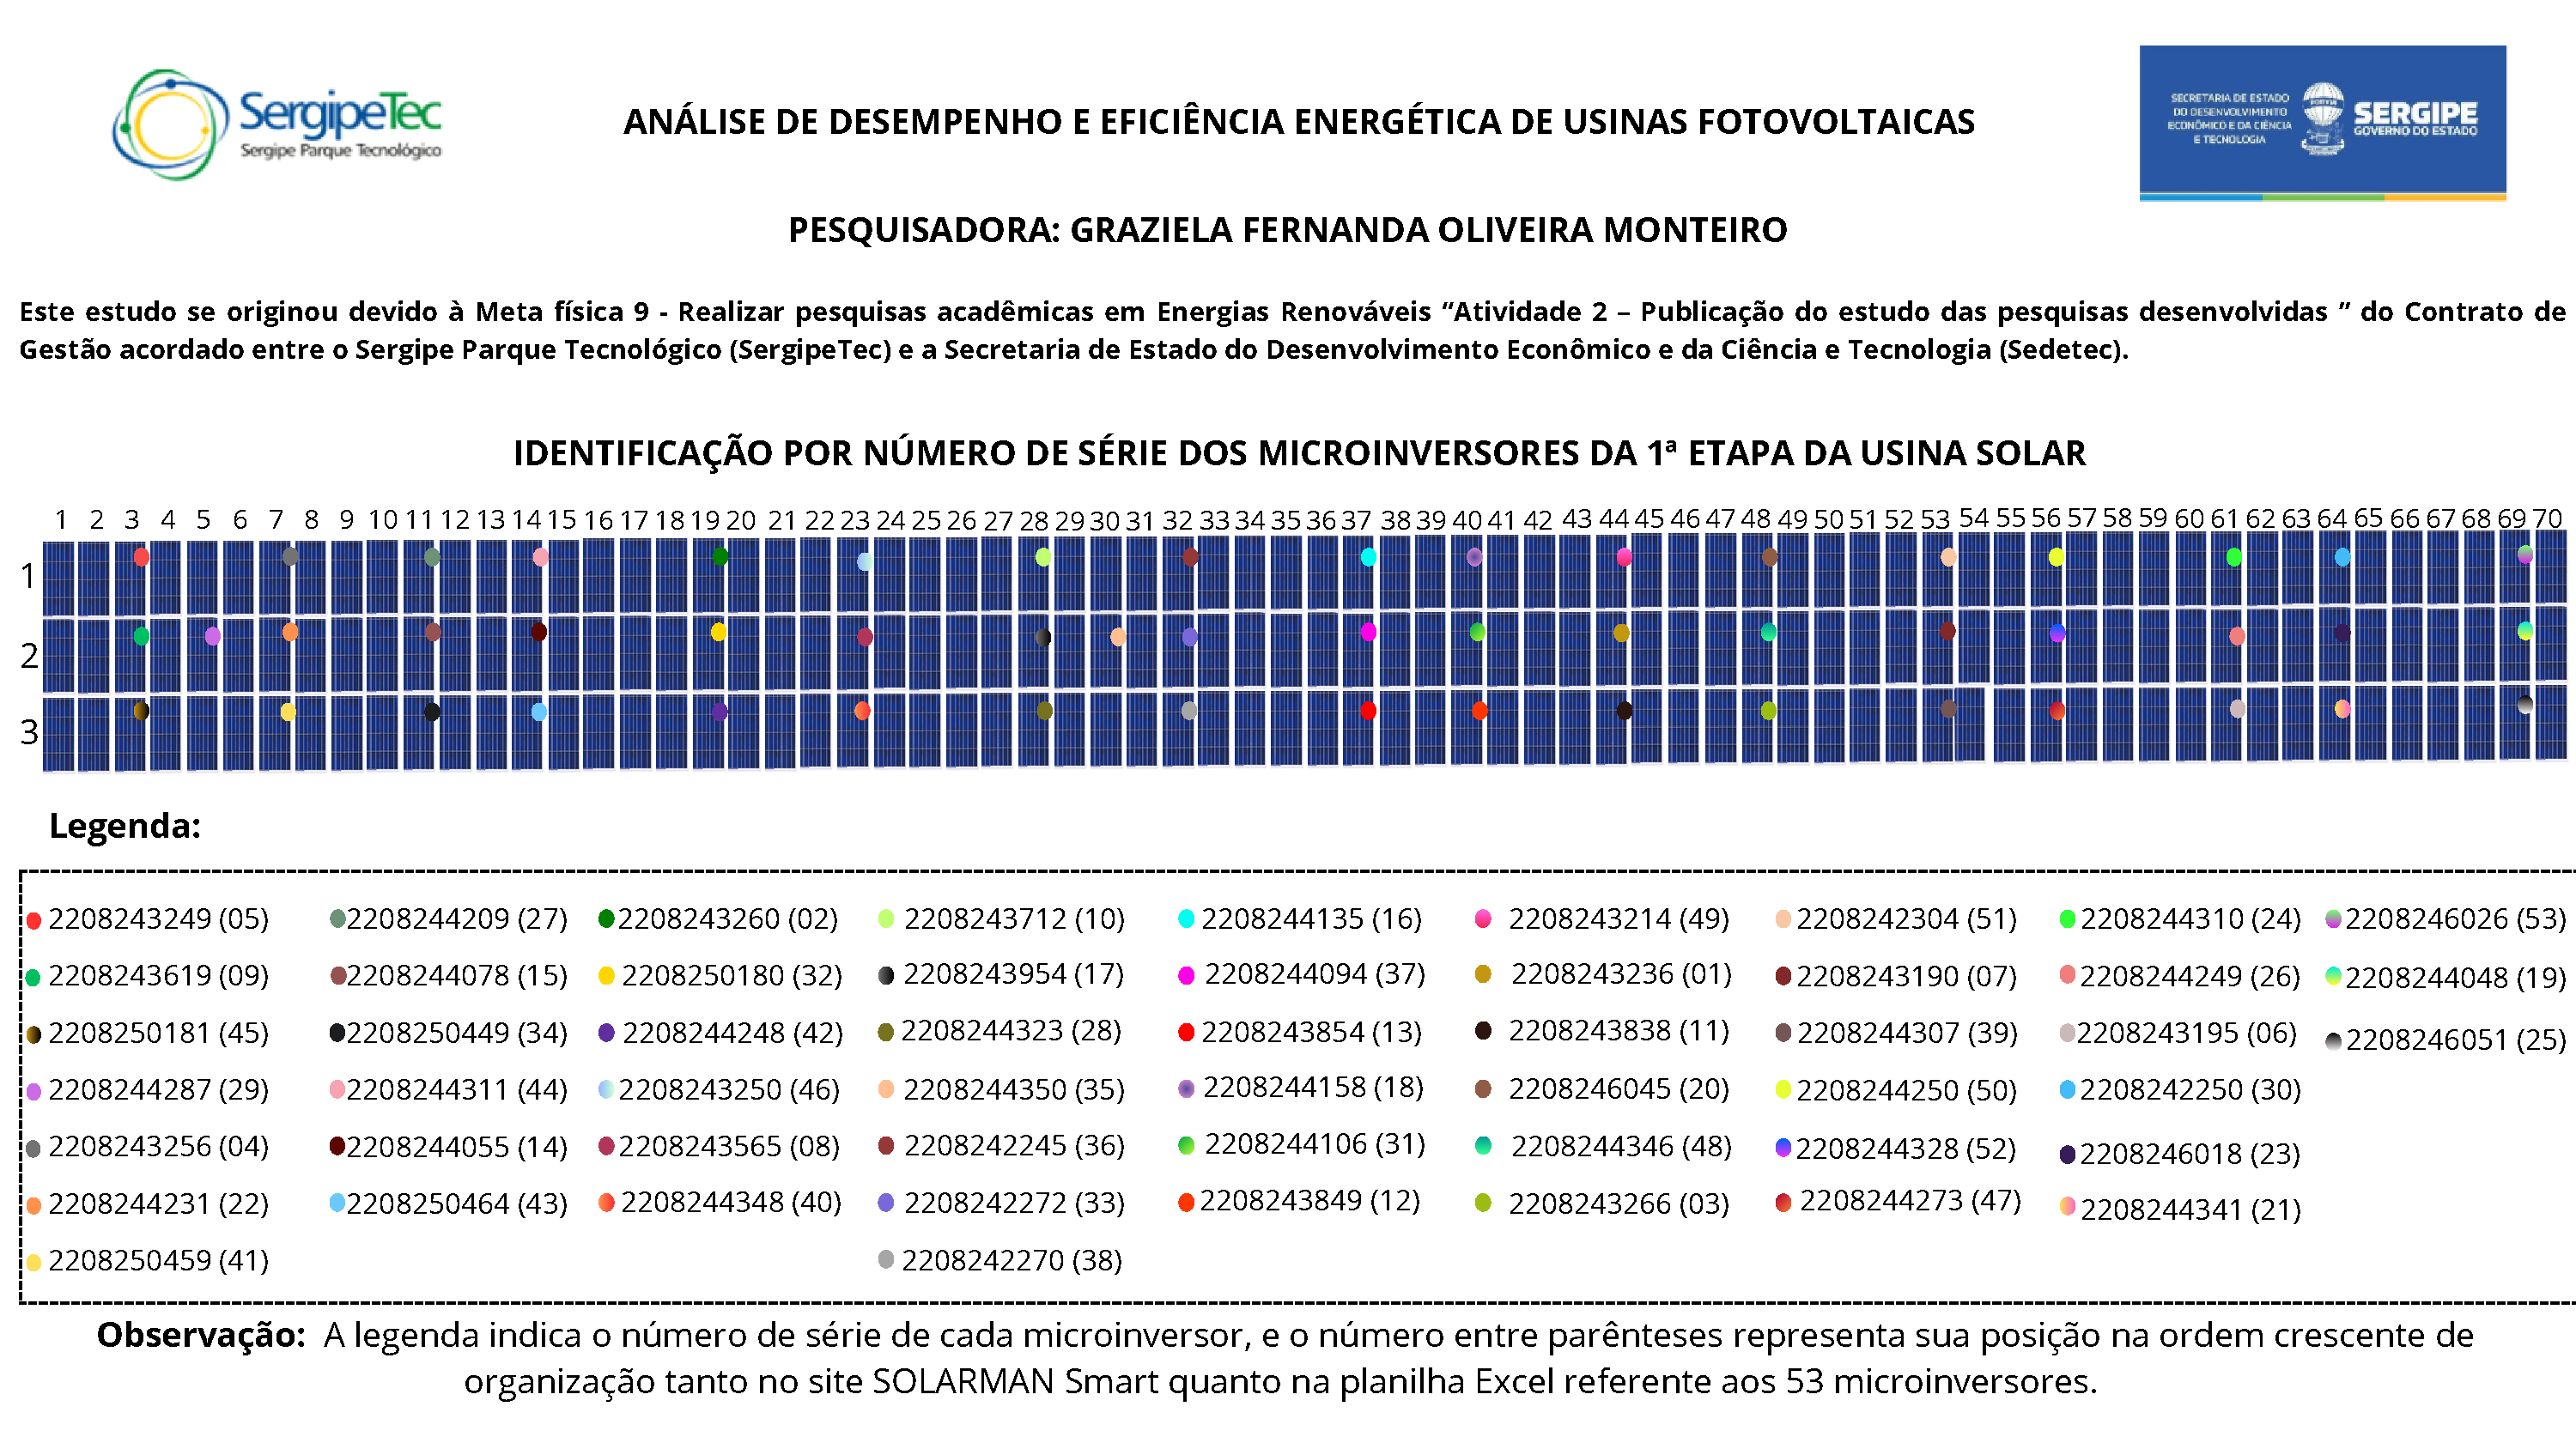
\includegraphics[page=1, width=\textwidth]{Anexos/CATALOGAÇÃO DA USINA SOLAR DO SERGIPETEC - 1ª ETAPA - GERAL.pdf}
        \caption{Exemplo de figura extraída do PDF — página 1}
        \label{fig:pdfpag1}
    \end{figure}
    
    % ---- restaurar o nome padrão ----
    \captionsetup[figure]{name=Figura}
    
    \begin{figure}[h!]
        \centering
        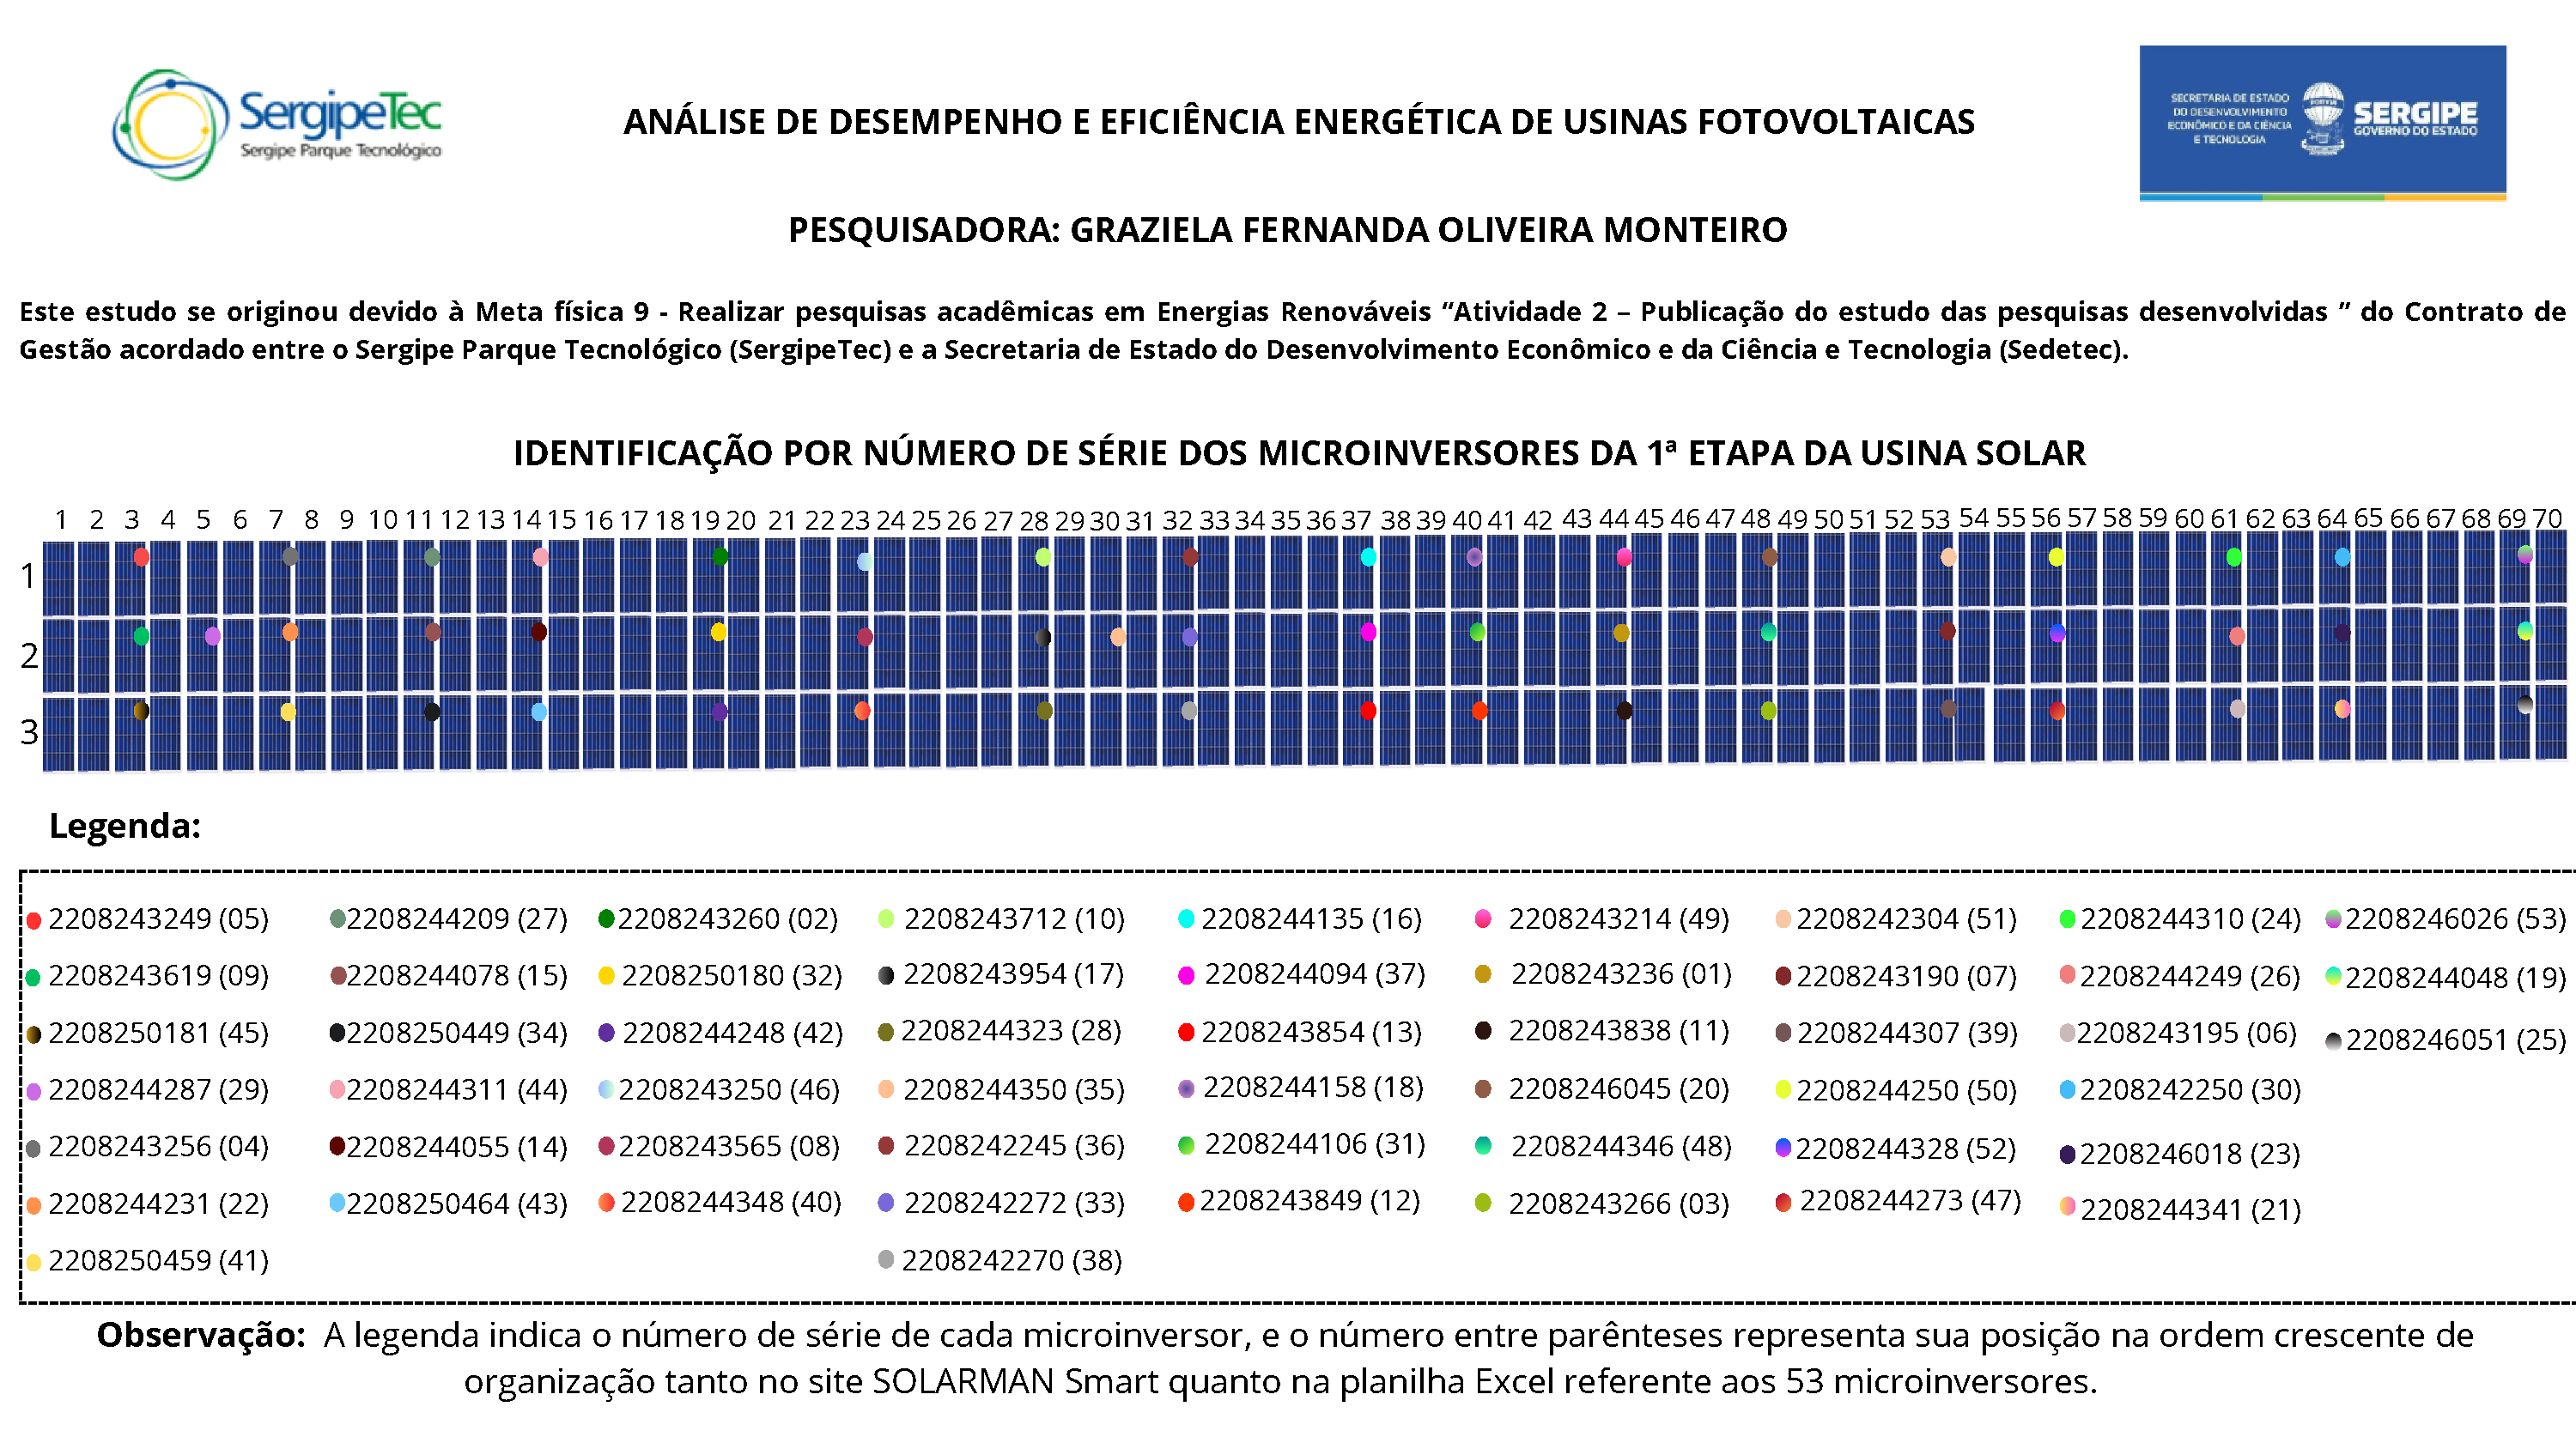
\includegraphics[page=1, width=0.9\textwidth]{Anexos/CATALOGAÇÃO DA USINA SOLAR DO SERGIPETEC - 1ª ETAPA - GERAL.pdf}
        \caption{Página 1 do PDF redimensionada}
        \label{fig:pdfpag2}
    \end{figure}

\end{comment}








\section{DIAGRAMA DE BLOCOS}

O diagrama de bloco mostra de forma simplificada toda a estrutura e os passos dessa dissertação, ilustrada na Figura 4.3: Diagrama de Blocos da Proposta de Dissertação.

\begin{figure}[H]
    \centering
    \caption{Diagrama de blocos da proposta de dissertação.}
    \includegraphics[width=5.0in]{Figuras/Fluxograma.pdf}
    \label{fig:Flux1}
    
    {\fontsize{10pt}{12pt}\selectfont
    \textbf{Fonte:} Próprio Autor, 2025}
\end{figure}


\renewcommand{\chaptername}{} % remove "Capítulo"
\chapter{RESULTADOS E DISCUSSÔES}
















 
\renewcommand{\chaptername}{} % remove "Capítulo"
\chapter{CRONOGRAMA DE ATIVIDADES}
%\addcontentsline{toc}{chapter}{CRONOGRAMA DE ATIVIDADES}

\label{sec:cronograma}
{\color{red}
O cronograma das atividades propostas para a realização deste trabalho é disposto na Figura \ref{fig:crono}, sendo elas:

\begin{itemize}
\justifying

    \item A1: Referencial teórico e revisão bibliográfica acerca de usinas solares carport, usina solares com microinversores e indicadores chave de desempenho (KPIs);
    \item A2: Mapeamento da usina de carport solar;
    \item A3: Monitoramento da usina e coleta de dados de geração via Solarman Smart;
    \item A4: Estudo da fundamentação teórica sobre indicadores chave de desempenho (KPIs);
    \item A5: Levantamento dos dados dos indicadores chave de desempenho (KPIs) em planilha Excel, preparação para cálculos de KPIs;
    \item A6: Cálculos dos indicadores chave de desempenho (KPIs), cálculo de payback e economia anual;
    \item A7: Levantamento das faturas de energia, através da coleta de informações durante um período de 1 ano antes e 1 ano após a primeira etapa da usina; 
    \item A8: Simulação de sombreamento (PV*SOL), modelagem 3D da usina, análise de sombreamento e impacto no desempenho;
    \item A9: Levantamento bibliográfico sobre energia solar, sombreamento, microinversores, KPIs, análises financeiras, usinas fotovoltaicas; 
    \item A10: Análise financeira e econômica, geração de gráficos de desempenho, KPIs por microinversor, gráficos financeiros (payback);
    \item A11: Geração de gráficos de KPIs (Excel e Power BI) e gráficos de retorno financeiro;
    \item A12: Relatório de eficiência; consolidação dos resultados técnicos e financeiros, análise final da usina;
    \item A13: Escrita da dissertação;
    \item A14: Defesa de dissertação.

\end{itemize}
}

%mudar a defesa para fevereiro
%empurrar a redacao do artigo para frente

\begin{figure}[H]
    \centering
    \caption{Cronograma de atividades previstas.}
    \label{fig:crono}
    \includegraphics[width=\textwidth]{Figuras/cronograma de atividades.pdf}
    
    {\fontsize{10pt}{12pt}\selectfont
    \textbf{Fonte:} Próprio Autor, 2025}
\end{figure}




 
% \input{Texto/6-resultados.tex}
\renewcommand{\chaptername}{} % remove "Capítulo"
\chapter{Conclusões}
%\addcontentsline{toc}{chapter}{CONSIDERAÇÕES FINAIS}
\label{cap:consideracoes}


Esta proposta de dissertação estrutura-se como um estudo abrangente sobre o desempenho, a eficiência energética e a viabilidade econômica da usina de carport solar já instalada no Sergipe Parque Tecnológico (SergipeTec), sendo as atividades executadas até o momento, as supracitadas no cronograma de atividades. Estas atividades forneceram uma base necessária para compreender o funcionamento do sistema e identificar parâmetros relevantes para as próximas fases da pesquisa.


Diante do que foi apresentado e por se tratar de uma pesquisa em andamento. As atividades subsequentes contemplam desde o aprofundamento teórico sobre indicadores chave de desempenho (KPIs), simulações de sombreamento em ambiente 3D via PV*SOL e levantamentos complementares de dados das faturas de energia, até a consolidação dos cálculos de eficiência energética, análises financeiras e geração dos principais KPIs por microinversor. A integração dos resultados técnicos e econômicos permitirá uma avaliação da performance da usina e do seu retorno energético e financeiro ao longo dos anos.

Em síntese, a elaboração dos gráficos e relatórios finais, bem como a análise consolidada de eficiência, constituirá um avanço significativo no estudo. Por fim, a fase de escrita da dissertação e a posterior defesa integrarão todas as evidências, cálculos, simulações e interpretações construídas ao longo de quase dois anos de pesquisa.

Assim, esta proposta de dissertação demonstra o avanço já alcançado até o momento e mostra o planejamento detalhado das atividades que ainda serão desenvolvidas até 2027. 






% \input{Texto/8-atividades.tex}
% \input{Texto/9-trabfuturos.tex}


\backmatter


\chapter*{REFERÊNCIAS BIBLIOGRÁFICAS}
\addcontentsline{toc}{chapter}{REFERÊNCIAS BIBLIOGRÁFICAS}


%\begin{thebibliography}{99}

\bibitem{Benedetti2020}
BENEDETTI, David; AGNELLI, Jacopo; GAGLIARDI, Alessio; DINI, Pierpaolo; SAPONARA, Sergio.
\textit{Design of an off-grid photovoltaic carport for a full electric vehicle recharging}.
In: \textbf{2020 IEEE International Conference on Environment and Electrical Engineering and 2020 IEEE Industrial and Commercial Power Systems Europe (EEEIC/I\&CPS Europe)}.
Anais [...]. IEEE, 2020. p. 1--6.


\bibitem{CRESESB}
CRESESB – CENTRO DE REFERÊNCIA PARA ENERGIA SOLAR E EÓLICA SÉRGIO BRITO.
\textit{CRESESB – Centro de Referência para Energia Solar e Eólica Sérgio Brito}.
Disponível em: https://www.cresesb.cepel.br. Acesso em: 25 nov. 2025.




\bibitem{Gulati2023}
GULATI, Himanshu; UPADHYAY, Prashant Kumar; REDDY, Yellasiri Bharath Kumar.
\textit{PV Plant Performance Review Methodology: Key Performance Indicators (KPI) Estimation}.
In: \textbf{2023 IEEE 50th Photovoltaic Specialists Conference (PVSC)}.
Anais [...]. IEEE, 2023. p. 1--4.

\bibitem{Kroth2020}
KROTH, Geovio; RAMPINELLI, Giuliano Arns.
\textit{Análise de indicadores de desempenho de um sistema fotovoltaico com distintos fatores de dimensionamento de inversor e diferentes ângulos azimutais}.
In: \textbf{Congresso Brasileiro de Energia Solar (CBENS)}.
Anais [...]. 2020.

\bibitem{Kulik2024}
KULIK, Ana Carolina.
\textit{Análise técnica e de desempenho do CARPORT instalado na UTFPR campus Neoville associado a diferentes veículos elétricos em Curitiba}.
2024. Dissertação (Mestrado) — Universidade Tecnológica Federal do Paraná, Curitiba, 2024.


\bibitem{Lakatos2009}
LAKATOS, Eva Maria; MARCONI, Marina de Andrade.
\textit{Metodologia científica}.
3. ed. São Paulo: Atlas, 2009.



\bibitem{Lindig2024}
LINDIG, Sascha et al.
\textit{Review of technical photovoltaic key performance indicators and the importance of data quality routines}.
\textbf{Solar RRL}, v. 8, n. 24, p. 2400634, 2024.

\bibitem{Odeh2018}
ODEH, Saad.
\textit{Analysis of the performance indicators of the PV power system}.
\textbf{Journal of Power and Energy Engineering}, v. 6, n. 6, p. 59--75, 2018.

\bibitem{Oliveira2021}
OLIVEIRA, Breno de.
\textit{Análise de desempenho através do cálculo de índices de mérito de sistemas fotovoltaicos conectados à rede}.
2021. Trabalho de Conclusão de Curso (Graduação em Engenharia Mecânica) — Universidade Federal de Sergipe, São Cristóvão, 2021.

\bibitem{Raimo2018}
RAIMO, Patricia Abdala; SOBREIRA, Rodrigo Leonel; BUENO, Edilson Aparecido.
\textit{Análise de desempenho da usina fotovoltaica de 70 kWp: estudo de caso do Instituto Federal — Campus São Paulo}.
In: \textbf{Congresso Brasileiro de Energia Solar (CBENS)}.
Anais [...]. 2018.

\bibitem{Rediske2024}
REDISKE, Graciele et al.
\textit{A proposed set of indicators for evaluating the performance of the operation and maintenance of photovoltaic plants}.
\textbf{Applied Energy}, v. 354, p. 122158, 2024.

\bibitem{Riakhi2021}
RIAKHI, Fatima-Ezzahra; KHALDOUN, Asmae.
\textit{PV sizing of a grid connected solar carport system linked to charging stations and its economic analysis}.
In: \textbf{9th International Renewable and Sustainable Energy Conference (IRSEC)}.
Anais [...]. IEEE, 2021. p. 1--6.

\bibitem{Santos2024}
SANTOS, Marcos Felipe Sobral dos et al.
\textit{Energia solar: um panorama sobre o estado de Sergipe}.
In: \textbf{Congresso Nacional de Engenharia de Petróleo, Gás Natural e Biocombustíveis}.
Anais [...]. Aracaju: Centro de Convenções de Sergipe, 2024.
Disponível em: https://www.even3.com.br/anais/vconepetro/810351-ENERGIA-SOLAR--UM-PANORAMA-SOBRE-O-ESTADO-DE-SERGIPE.
Acesso em: 28 nov. 2025.


\bibitem{SilvaFausto2022}
SILVA, Fausto Batista Felix; SILVEIRA, Nicolli Sperança.
\textit{Análise de desempenho de carports com diferentes tecnologias fotovoltaicas}.
In: \textbf{Congresso Brasileiro de Energia Solar (CBENS)}.
Anais [...]. 2022. p. 1--7.

\bibitem{SilvaRaquel2022}
SILVA, Raquel Xavier.
\textit{Análise de desempenho de usina solar fotovoltaica utilizando simulações com dados de entrada medidos}.
2022.

\bibitem{Theocharides2024}
THEOCHARIDES, Spyros et al.
\textit{Characterization of voltage fluctuations: a methodology to KPI analysis and anomaly diagnosis}.
In: \textbf{3rd International Conference on Energy Transition in the Mediterranean Area (SyNERGY MED)}.
Anais [...]. IEEE, 2024. p. 1--6.

\bibitem{Yalawar2018}
YALAWAR, Akshata; NAYAK, Shravankumar.
\textit{Evaluation of performance parameters and economic analysis of 1 MW grid connected solar PV plant}.
In: \textbf{4th International Conference for Convergence in Technology (I2CT)}.
Anais [...]. IEEE, 2018. p. 1--5.

%\end{thebibliography}





% ----- APÊNDICE 1 - CATALOGAÇÃO DA USINA SOLAR -----
\clearpage % garante que começa em página nova
\phantomsection % marca link para o sumário correto
\label{ap:catalogacao-u}
\addcontentsline{toc}{chapter}{APÊNDICE 1 - CATALOGAÇÃO DA USINA SOLAR} % adiciona ao sumário



\vspace*{\fill} % centraliza verticalmente
\begin{center}
    {\LARGE \textbf{APÊNDICE 1}}\\[1\baselineskip]
    {\LARGE \textbf{CATALOGAÇÃO DA USINA SOLAR}}
\end{center}
\vspace*{\fill}




\clearpage % próxima página começa depois do anexo

%\section*{Conteúdo do Anexo}
%\addcontentsline{toc}{section}{Conteúdo do Anexo} % se quiser adicionar subtítulo ao sumário
%Aqui vai o conteúdo do anexo, imagens, figuras, tabelas etc.

%\captionsetup[figure]{name=Anexo} % muda o nome apenas para a próxima figura

\begin{figure}[h!]
\centering
\hspace*{-2.7cm}
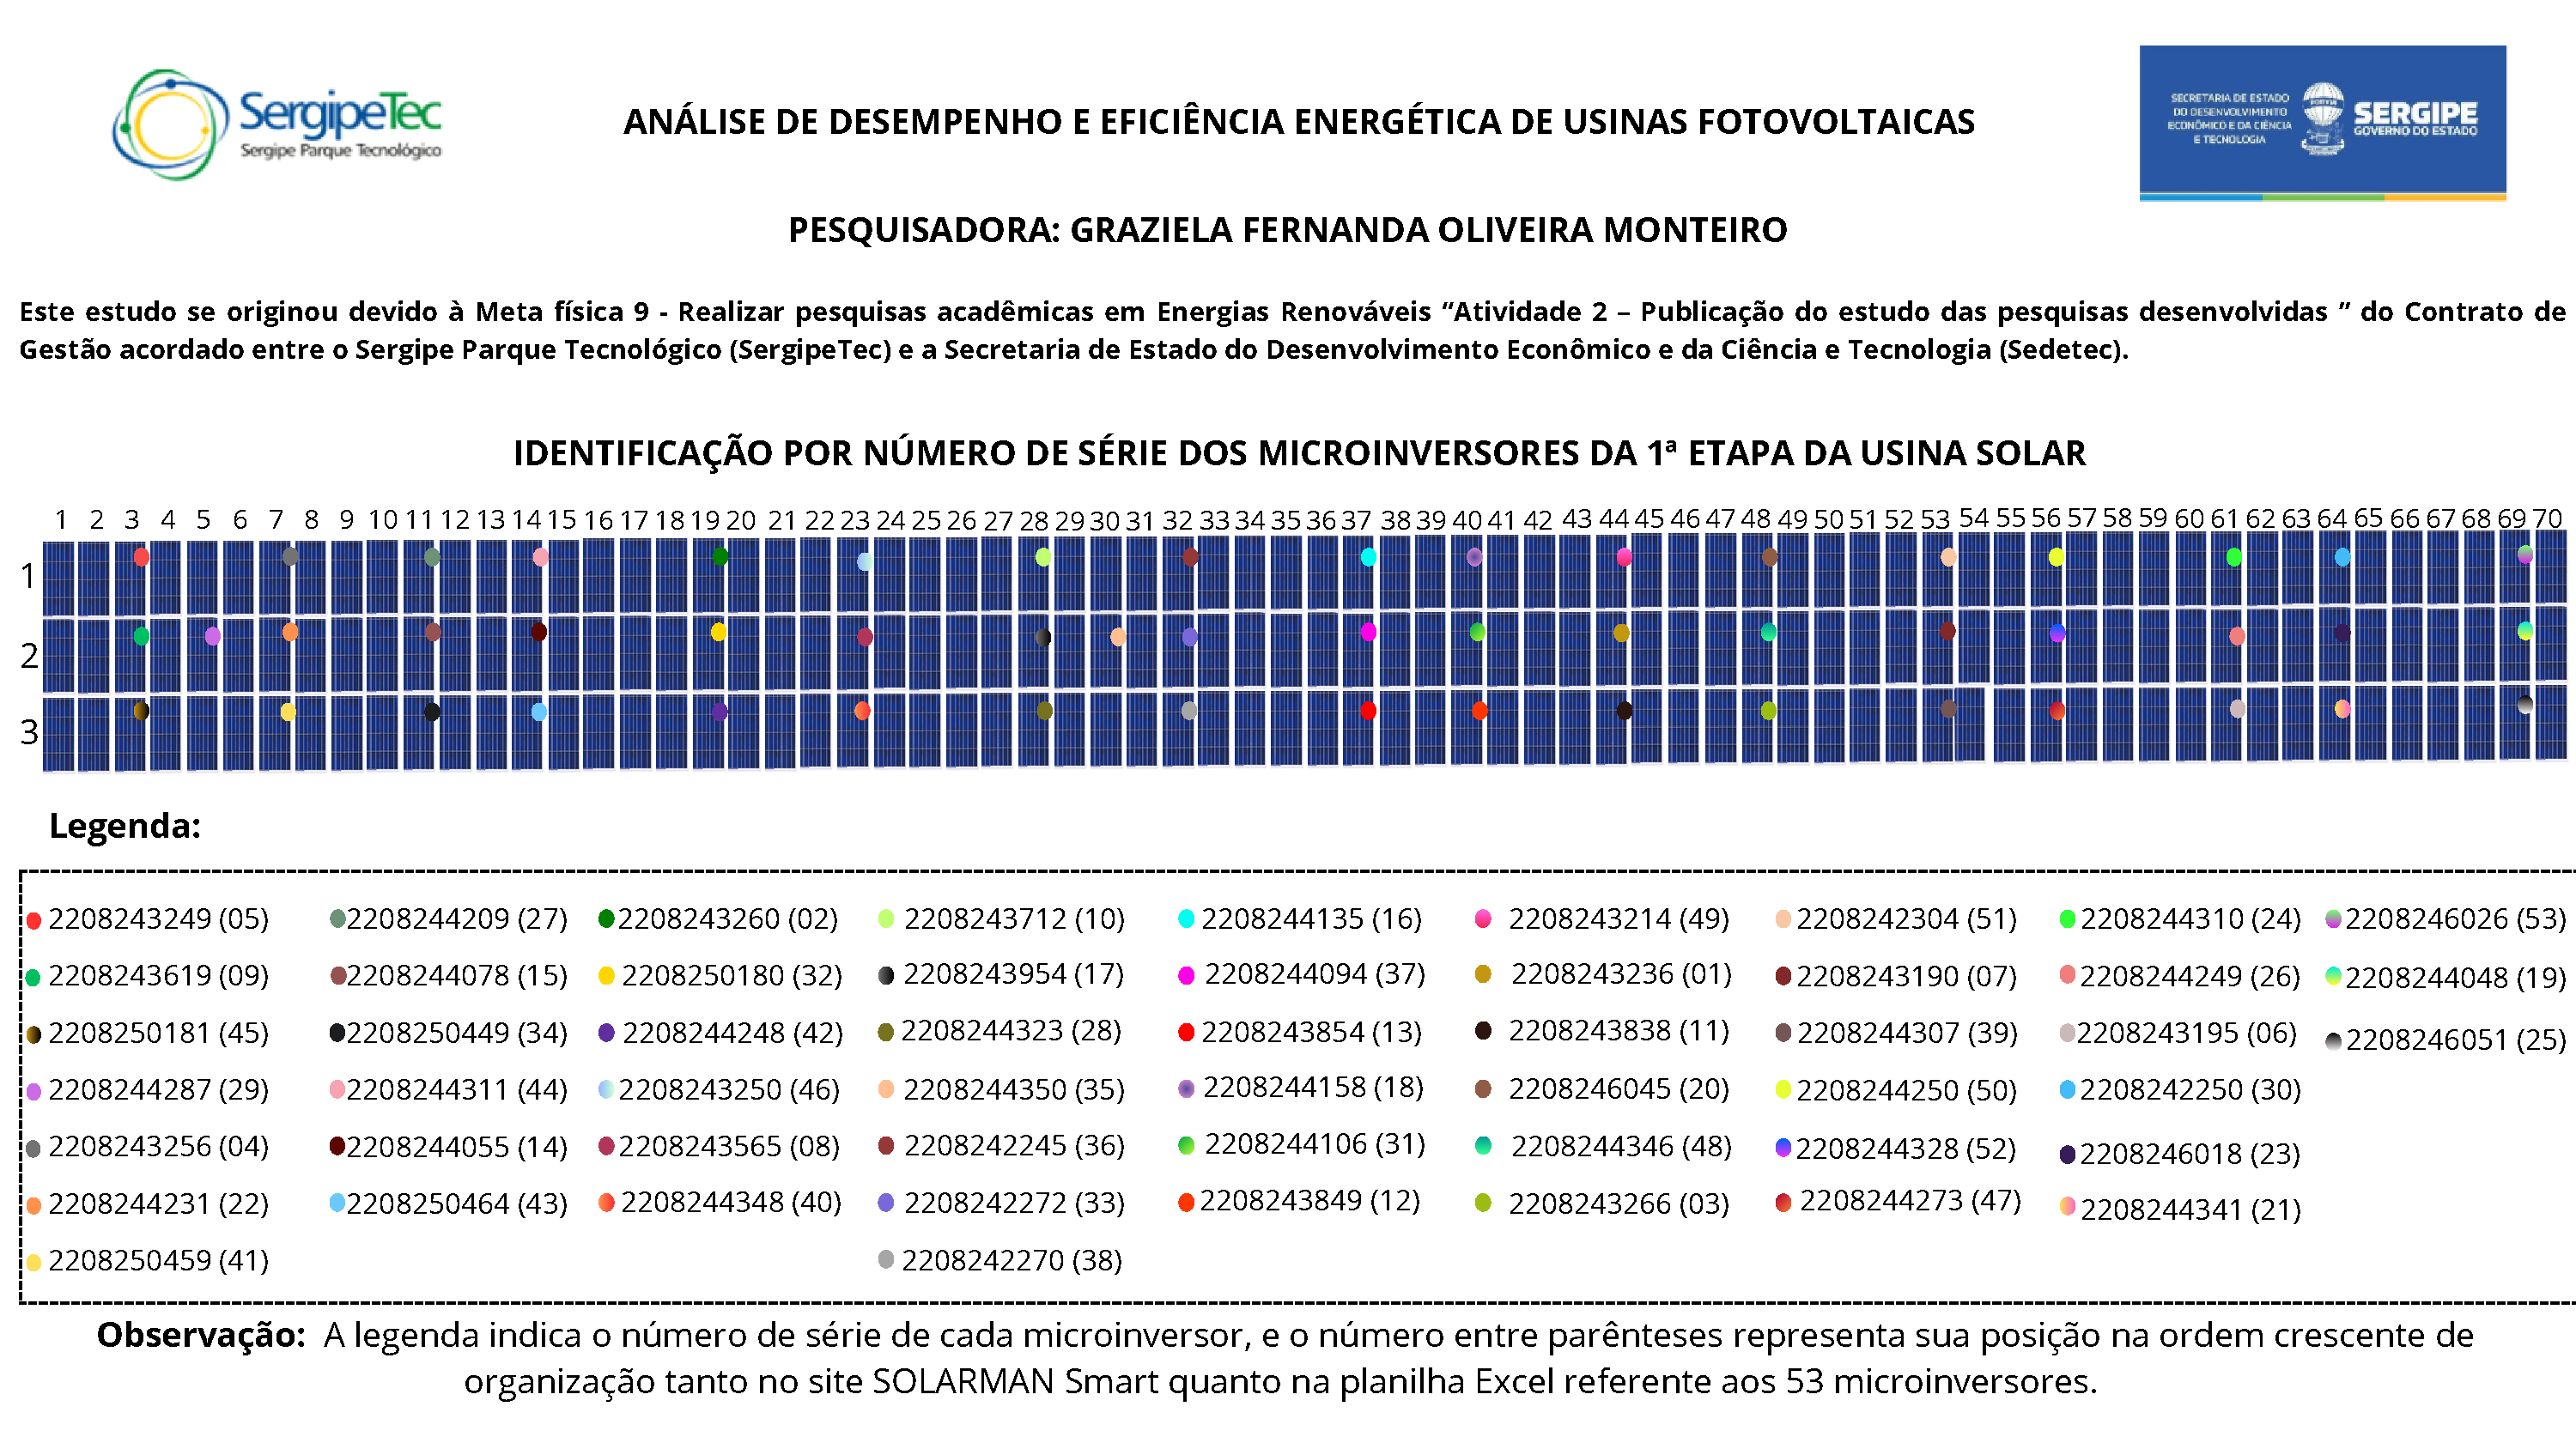
\includegraphics[page=1, width=1.25\textwidth]{Anexos/CATALOGAÇÃO DA USINA SOLAR DO SERGIPETEC - 1ª ETAPA - GERAL.pdf}
\caption*{}
\label{fig:pdfpag1}
\end{figure}




% ---- restaurar o nome padrão ----
\captionsetup[figure]{name=Figura}

\begin{figure}[h!]
    \centering
    \vspace{-1cm}
    \hspace*{-2.7cm}
    \includegraphics[page=2, width=1.25\textwidth]{Anexos/CATALOGAÇÃO DA USINA SOLAR DO SERGIPETEC - 1ª ETAPA - GERAL.pdf}
    \caption*{}
    \label{fig:pdfpag2}
\end{figure}

\begin{figure}[h!]
    \centering
    \hspace*{-2.7cm}
    \includegraphics[page=3, width=1.25\textwidth]{Anexos/CATALOGAÇÃO DA USINA SOLAR DO SERGIPETEC - 1ª ETAPA - GERAL.pdf}
    \caption*{}
    \label{fig:pdfpag3}
\end{figure}

\begin{figure}[h!]
    \centering
    \hspace*{-2.7cm}
    \includegraphics[page=4, width=1.25\textwidth]{Anexos/CATALOGAÇÃO DA USINA SOLAR DO SERGIPETEC - 1ª ETAPA - GERAL.pdf}
    \caption*{}
    \label{fig:pdfpag4}
\end{figure}

\clearpage
\vspace*{-\topskip}
\begin{center}
    \hspace*{-2.7cm}
    \includegraphics[page=5, width=1.25\textwidth]{Anexos/CATALOGAÇÃO DA USINA SOLAR DO SERGIPETEC - 1ª ETAPA - GERAL.pdf}
\end{center}






























% ----- ANEXO 1 - Manual e datasheet do carport solar -----
\clearpage % garante que começa em página nova
\phantomsection % marca link para o sumário correto
\label{ap:datasheet-carport}
\addcontentsline{toc}{chapter}{ANEXO 1 - MANUAL E DATASHEET DO CARPORT SOLAR} % adiciona ao sumário



\vspace*{\fill} % centraliza verticalmente
\begin{center}
    {\LARGE \textbf{ANEXO 1}}\\[1\baselineskip]
    {\LARGE \textbf{MANUAL E DATASHEET DO CARPORT SOLAR}}

    
\end{center}
\vspace*{\fill}




\newpage % próxima página começa depois do anexo

%section*{Conteúdo do Anexo}
%addcontentsline{toc}{section}{Conteúdo do Anexo} % se quiser adicionar subtítulo ao sumário
%Aqui vai o conteúdo do anexo, imagens, figuras, tabelas etc.

\captionsetup[figure]{name=Anexo} % muda o nome apenas para a próxima figura

    \vspace*{0cm}
    \centering
    \hspace*{-1.5cm}
    \includegraphics[page=1, width=1.1\textwidth]{Anexos/Manual - Garagem - Carport Solar RS-401 .pdf}
    \label{fig:pdfpag1}


    
    \vspace*{-2cm}
    \centering
    \hspace*{-1.5cm}
    \includegraphics[page=2, width=1.1\textwidth]{Anexos/Manual - Garagem - Carport Solar RS-401 .pdf}
    \label{fig:pdfpag1}


    \vspace*{-2cm}
    \centering
    \hspace*{-1.5cm}
    \includegraphics[page=3, width=1.1\textwidth]{Anexos/Manual - Garagem - Carport Solar RS-401 .pdf}
    \label{fig:pdfpag1}



    \vspace*{-2cm}
    \centering
    \hspace*{-1.5cm}
    \includegraphics[page=4, width=1.1\textwidth]{Anexos/Manual - Garagem - Carport Solar RS-401 .pdf}
    \label{fig:pdfpag1}




\begin{figure}[h!]
    \centering
    \hspace*{-2.7cm}
    \includegraphics[page=1, width=1.25\textwidth]{Anexos/RS-401 (CLIENTE).pdf}
    \caption*{}
    \label{fig:pdfpag1}
\end{figure}


\begin{figure}[h!]
    \centering
    \hspace*{-2.7cm}
    \includegraphics[page=2, width=1.25\textwidth]{Anexos/RS-401 (CLIENTE).pdf}
    \caption*{}
    \label{fig:pdfpag1}
\end{figure}



\begin{figure}[h!]
    \centering
    \hspace*{-2.7cm}
    \includegraphics[page=3, width=1.25\textwidth]{Anexos/RS-401 (CLIENTE).pdf}
    \caption*{}
    \label{fig:pdfpag1}
\end{figure}


\begin{figure}[h!]
    \centering
    \hspace*{-2.7cm}
    \includegraphics[page=4, width=1.25\textwidth]{Anexos/RS-401 (CLIENTE).pdf}
    \caption*{}
    \label{fig:pdfpag1}
\end{figure}














% ----- ANEXO 2 - DATASHEET DOS MÓDULOS FOTOVOLTAICOS -----
\clearpage % garante que começa em página nova
\phantomsection % marca link para o sumário correto
\label{ap:datasheet-modulos}
\addcontentsline{toc}{chapter}{ANEXO 2 - DATASHEET DOS MÓDULOS FOTOVOLTAICOS} % adiciona ao sumário



\vspace*{\fill} % centraliza verticalmente
\begin{center}
    {\LARGE \textbf{ANEXO 2}}\\[1\baselineskip]
    {\LARGE \textbf{DATASHEET DO MÓDULO FOTOVOLTAICO}}
\end{center}
\vspace*{\fill}




\clearpage % próxima página começa depois do anexo

%\section*{Conteúdo do Anexo}
%\addcontentsline{toc}{section}{Conteúdo do Anexo} % se quiser adicionar subtítulo ao sumário
%Aqui vai o conteúdo do anexo, imagens, figuras, tabelas etc.

%\captionsetup[figure]{name=Anexo} % muda o nome apenas para a próxima figura

\clearpage
\vspace*{-2cm}
\centering
\hspace*{-2.0cm}
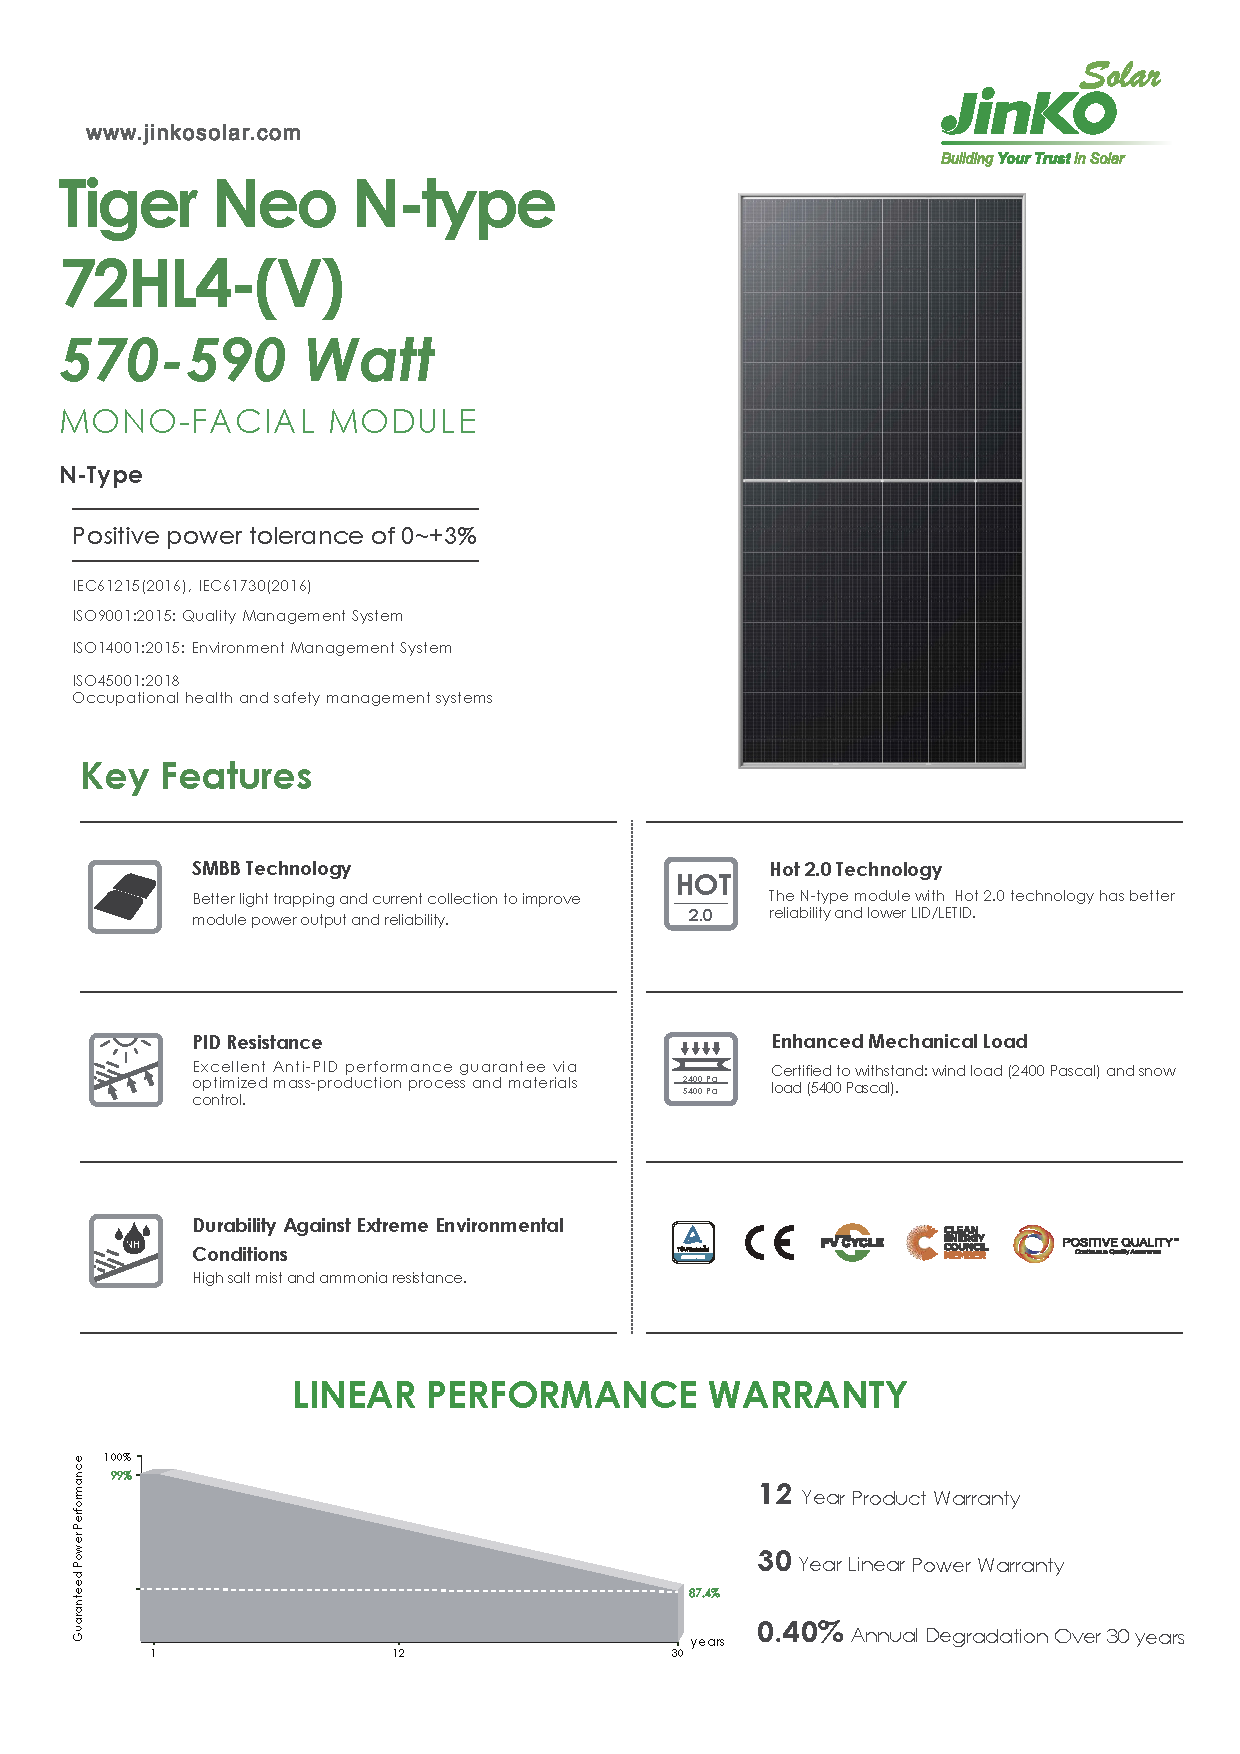
\includegraphics[page=1, width=1.15\textwidth]{Anexos/DATASHEET- JINKO 580W.pdf}
\label{fig:pdfpag1}




\vspace*{-2cm}
\centering
\hspace*{-2.0cm}
\includegraphics[page=2, width=1.15\textwidth]{Anexos/DATASHEET- JINKO 580W.pdf}
\label{fig:pdfpag1}

















% ----- ANEXO 3 - DATASHEET DOS MICROINVERSORES -----
%\newpage % garante que começa em página nova
\phantomsection % marca link para o sumário correto
\label{ap:datasheet-microinversores}
\addcontentsline{toc}{chapter}{ANEXO 3 - DATASHEET DOS MICROINVERSORES} % adiciona ao sumário



\vspace*{\fill} % centraliza verticalmente
\begin{center}
    {\LARGE \textbf{ANEXO 3}}\\[1\baselineskip]
    {\LARGE \textbf{DATASHEET DO MICROINVERSOR}}
\end{center}
\vspace*{\fill}




\clearpage % próxima página começa depois do anexo

%\section*{Conteúdo do Anexo}
%\addcontentsline{toc}{section}{Conteúdo do Anexo} % se quiser adicionar subtítulo ao sumário
%Aqui vai o conteúdo do anexo, imagens, figuras, tabelas etc.

%\captionsetup[figure]{name=Anexo} % muda o nome apenas para a próxima figura

\begin{figure}[h!]
    \centering
    \hspace*{-2.7cm}
    \includegraphics[page=1, width=1.25\textwidth]{Anexos/DATASHEET - MICROINVERSOR DEYE 2kW.pdf}
    \caption*{}
    \label{fig:pdfpag1}
\end{figure}

















\end{document}

